%%%%%%%%%%%%%%%%%%%%%%%%%%%%%%%%%%%%%%%%%%%%%%%%%%%%%%%%%%%%%%%%%%%
%                                                                 %
%                      Thesis root file                           %
%                                                                 %
%%%%%%%%%%%%%%%%%%%%%%%%%%%%%%%%%%%%%%%%%%%%%%%%%%%%%%%%%%%%%%%%%%%

%\documentclass[chapter,a4paper]{rmdthesis}
\documentclass[chapter,a4paper,openright,oneside]{uwchonoursthesis}
% Use the first command below if you want captions over 1 line indented. A side
% effect of this is to remove the use of bold for captions. To restore bold,
% also include the second line below.
%\usepackage[hang]{caption}      % to indent subsequent lines of captions
\usepackage{natbib}
\usepackage{color}              % to use color such as \textcolor{red}{this is red}
\usepackage{verbatim}
\usepackage{graphicx}
\usepackage{float}
\usepackage{caption}
\usepackage{amsmath}
\usepackage{subcaption}
\graphicspath{figures}          % sets paths to figures subdirectory
                                % to use 
                                % \includegraphics{thefigure} 
                                % instead of 
                                % \includegraphics{figures/thefigure} 
\usepackage{flafter}
\usepackage{amsfonts}
\usepackage{rotating}
\usepackage{url}
\usepackage{setspace}
\usepackage{pstricks}
\usepackage{pstricks-add}

% \renewcommand{\captionfont}{\bfseries} % bold caption (needed with caption
                                       % package; otherwise bold is default)

%\includeonly{4chapter}  % use \includeonly to process only
                         % the file(s) listed inside the braces
%\includeonly{title}     % use \includeonly to process title only
                         % use this when you fiddle with the style of the title

\usepackage{makeidx}
\makeindex      % put before \begin{document}
                % examples of indexed terms appear in 1chapter
%\printindex    % put where you want index

% \renewcommand{\cite}{\citep}
\begin{document}

%
% start of frontstuff
%

%frontstuff       % this can be a command

%%%%%%%%%%%%%%%%%%%%%%%%%%%%%%%%%%%%%%%%%%%%%%%%%%%%%%%%%%%%%%%%%%%
%                                                                 %
%                              Title page                         %
%                         Master's Thesis at UWC                  %
%                                  or                             %
%                         Honour's Thesis at UWC                  %
%                                                                 %
%%%%%%%%%%%%%%%%%%%%%%%%%%%%%%%%%%%%%%%%%%%%%%%%%%%%%%%%%%%%%%%%%%%

% Supply information for use on title page:
%\thesistitle{The influence of interfaces on the understanding of 
% mathematics in secondary schools in Afghanistan} 
\thesistitle{Automatic Human Emotion Detection} 
%The Title of Your Thesis % \\
%                 Note the Capitalization of Some of the %\\*[6pt]
%                 Words in the Title}
% Do NOT insert newline commands such as \\ or \\*[6pt] because 
% this title is used in your Declaration which is  automaticaly 
% generated from the \title{...} and \author{...} information.
\author{Retshidisitswe Lehata}

% You may put in your middle names or their initials here 
\degree{Bachelor of Science Honours} 
                                        
\supervisor{Mehrdad Ghaziasgar}    % For M.Sc. at UWC 
\cosupervisor{Reg Dodds}           % For M.Sc. at UWC 
%\promotor{For Ph.D.s only}        % For Ph.D. at UWC 
%              This requires editing the style sheet.

\submitdate{October 2016}          % \submitdate is like an assignment
\submitdate{This version \today}   % the last \submitdate is printed.

%\copyrightyear{2007}   % if omitted, current year is used.
% Copyright is not appropriate at UWC, since you have
% signed away your copyright rights to the University.

% Print titlepage and other prefatory material:
\titlepage
   % titlepage material for Honour's, Master's thesis or project
%%%%%%%%%%%%%%%%%%%%%%%%%%%%%%%%%%%%%%%%%%%%%%%%%%%%%%%%%%%%%%%%%%%%
%                                                                 %
%                              Title page                         %
%                         Master's Thesis at UWC                  %
%                                  or                             %
%                         Honour's Thesis at UWC                  %
%                                                                 %
%%%%%%%%%%%%%%%%%%%%%%%%%%%%%%%%%%%%%%%%%%%%%%%%%%%%%%%%%%%%%%%%%%%

% Supply information for use on title page:
%\thesistitle{The influence of interfaces on the understanding of 
% mathematics in secondary schools in Afghanistan} 
\thesistitle{Automatic Human Emotion Detection} 
%The Title of Your Thesis % \\
%                 Note the Capitalization of Some of the %\\*[6pt]
%                 Words in the Title}
% Do NOT insert newline commands such as \\ or \\*[6pt] because 
% this title is used in your Declaration which is  automaticaly 
% generated from the \title{...} and \author{...} information.
\author{Retshidisitswe Lehata}

% You may put in your middle names or their initials here 
\degree{Bachelor of Science Honours} 
                                        
\supervisor{Mehrdad Ghaziasgar}    % For M.Sc. at UWC 
\cosupervisor{Reg Dodds}           % For M.Sc. at UWC 
%\promotor{For Ph.D.s only}        % For Ph.D. at UWC 
%              This requires editing the style sheet.

\submitdate{October 2016}          % \submitdate is like an assignment
\submitdate{This version \today}   % the last \submitdate is printed.

%\copyrightyear{2007}   % if omitted, current year is used.
% Copyright is not appropriate at UWC, since you have
% signed away your copyright rights to the University.

% Print titlepage and other prefatory material:
\titlepage
  % titlepage material for PhD thesis
%%%%%%%%%%%%%%%%%%%%%%%%%%%%%%%%%%%%%%%%%%%%%%%%%%%%%%%%%%%%%%%%%%%
%                                                                 %
%                            ABSTRACT                             %
%                                                                 %
%%%%%%%%%%%%%%%%%%%%%%%%%%%%%%%%%%%%%%%%%%%%%%%%%%%%%%%%%%%%%%%%%%%
\specialhead{Abstract}

Customer service is a large revenue stream for some companies, therefore ensuring that they provide the best quality service is likely to be their main priority. Not all customers readily express their emotions, verbally, regarding the quality of the service they are provided. Mehrabian 1980, states that 55\% of communication is facial expression. The motivation for this project is to apply an Automatic Human Emotion Detection(AHED) system in cases where an employee interacts with a customer. The AHED system focuses on emotion recognition using facial expressions. The proposed method for this project, first captures an image from the camera, the image is processed using the Viola Jones Algorithm to detect the face and the Histogram of Oriented Gradients(HOG) to extract the features from the face. Lastly the AHED system is trained using Support Vector Machines(SVM), to classify each emotion. There are six universal human expressions described by Ekman and Friesen, namely Surprise, Fear, Disgust, Anger, Happiness and Sadness. Grayscale frontal images will be used as input for the AHED system.

%\openpage
%%%%%%%%%%%%%%%%%%%%%%%%%%%%%%%%%%%%%%%%%%%%%%%%%%%%%%%%%%%%%%%%%%%%
%                                                                 %
%                          Key words                              %
%                                                                 %
%%%%%%%%%%%%%%%%%%%%%%%%%%%%%%%%%%%%%%%%%%%%%%%%%%%%%%%%%%%%%%%%%%%

\specialhead{Key words}

\vspace{12pt}

e-learning\\*[+12pt]
secondary schools\\*[+12pt]
Computer Aided Instruction\\*[+12pt]
Internet\\*[+12pt]
ANGeL\\*[+12pt]
set theory\\*[+12pt]
mother tongue\\*[+12pt]
gender\\*[+12pt]
Graphical User Interface\\*[+12pt]
Human Computer Interaction\\*[+12pt]
user interface design\\*[+12pt]
visual programming


%\openpage
%                         Acknowledgement

\specialhead{Acknowledgment}

This thesis is a compilation of the efforts of many people that helped and
me through the years. I would first like to thank my supervisor Mehrdad Ghaziasgar and co-supervisor Regg Dodds for encouraging me during my study. Without our weekly meetings, this work
would not have been possible. 
%At this time I would like to extend a very
%special thanks to the post-graduate assistant .  Without their help I would
%certainly not be where I am today.

%I would also like to thank the Trustees of Blanketyblank for their unwavering
%financial assistance without which my efforts would have been impossible.

%\openpage
\tableofcontents
%\listoftables          %required if there are tables
\listoffigures         %required if there are figures
%\openpage
%%                            Glossary                             %

\specialhead{Glossary}

\begin{description}
\item[\textbf{ACCC}] Afghan Canadian Community Centre.
\item[\textbf{Action Script}] is an object-oriented programming language 
for creating customized web-based learning aids.  Action script 
is a language that allows the creation of web-based games and rich 
Internet applications with streaming media such as video and audio. 
\item[\textbf{ANGeL}]  Afghan Next Generation environment for Learning is an 
e-learning environment adapted from KEWL for Afghanistan.
\item[\textbf{CHI}] Computer Human Interaction.  Computer scientists 
deal with the hardware and software that drive the interface and 
thus put the computer before the human, namely, CHI.
\item[\textbf{CSV}] Comma separated variables.
\item[\textbf{ERTV}] Educational Radio and Television.
\item[\textbf{FLASH}]  is an abbreviation for Adobe, Shockwave or Macromedia 
Flash.  It is a set of multimedia technologies first introduced 
in 1996 that has become a popular method for adding animation 
and interactivity to web pages. It is also used to develop rich Internet 
applications~\cite{allaire02}.
\item[\textbf{HCI}] Human Computer Interaction. It is the physical and mental 
boundary between users and input/output devices of a computer. All 
interactive computer processes require that a human gives some instruction 
to the computer, e.g. to store data, and receives feedback from the computer.
\item[\textbf{Informant Design}] is a framework used to involve various participants 
in the design process. ``It allows making maximal use of the input 
of the participants at different stages of the design''~\cite{scaife97}.
%(Michael Scaife 1997). 
\item[\textbf{KEWL}] Knowledge Environment for Web-based Learning.  An e-learning 
management system developed at the University of the Western Cape, 
South Africa.
\item[\textbf{Participatory Design}]  Is an approach that respects users as 
partners in the design process and ``in doing so explicitly gives them 
a more equal and responsible role''~\cite{scaife97}.
%(Michael Scaife 1997).
% \item[\textbf{UWC}]  The University of the Western Cape.
\item[\textbf{UNESCO}] United Nations Educational, Scientific and Cultural Organization.
\item[\textbf{UNICEF}] The United Nations Children's Fund.
\item[\textbf{USAID}] United States Agency for International Development.

\end{description}



%end of frontstuff


\chapter{Introduction}


Communication plays a large role, in daily human interaction. It can take the form of verbal or non-verbal communication, Mehrabian found that over 93\% of verbal communication is conveyed through ones tone of voice, 38\%,  and non-verbal ques, 55\% \cite{mehrabian}. Understanding non-verbal communication is a valuable skill, in that it is a universal form of communication. 
%Verbal communication is conveyed through ones tone voice, non-verbal ques and word construction. According to Mehrrabian tone of voice and non-verbal ques account for approximately 93\%. 
Non-verbal communication is a combination of body language, physical gestures and facial expressions. Ekman \& Friesen found six facial expressions that are universally identifiable in recognizing Fear, Anger, Disgust, Surprise, Happiness and Sadness \cite{ekman}. A facial expression is made up of the changes in facial muscles mainly the mouth, eyes and eyebrows. These changes help to reflect one’s current state of mind. 
\newline
The rest of this chapter is organised as follows: Section 1.1 describes the problem statement; Section 1.2 provides the overview of the solution proposed in this project and Section 1.3 outlines the method of implementing the proposed solution.

\section{Problem Statement}
Companies use feedback from their customers as a metric to measure their customer satisfaction rate. Customer feedback can be initiated by the customer as a compliment or criticism, based on the service they were given. Alternatively, a company can offer their customers optional online or physical surveys to be completed. The problem is that customers are more likely to refrain from commenting on a service, unless provoked to do so. Customer service is a large revenue stream for companies whose core business is based around the customer. Ensuring that the customer stays happy is key, for their success. 

\section{Proposed Solution}
An Automatic Human Emotion Detection system can be applied in any environment that benefits from understanding facial expressions and human emotion.
The proposed solution combines customer satisfaction with an automated system. This is done by using face detection to find the customers face in an image and facial feature extraction to identify the dominant customer emotion features in that image. To get the best results possible the training and classification of the system will be done using a machine learning technique. Companies can later incorporate the results of the system in improving their customer service, ensuring that their customers stay satisfied.

\section{Proposed Method}
A grayscale frontal image of the customer is used as input for the system. The Viola Jones Algorithm is then used to detect the location of the face in the image and the Histogram of Oriented Gradients is used to extract the features. Lastly the AHED system is trained using Support Vector Machines, to classify each emotion.


\chapter{Related Work}

There are a wide variety of methods that are used in the field of emotion recognition using facial expressions. However, a large number of those methods are implemented using a similar process. Shown in Figure ~\ref{fig:process}, initially the image is captured and processed. Thereafter the face is detected and features are extracted. Then a machine learning technique is trained to do the classification of the emotions. 

\begin{figure}[ht]
  \centering
  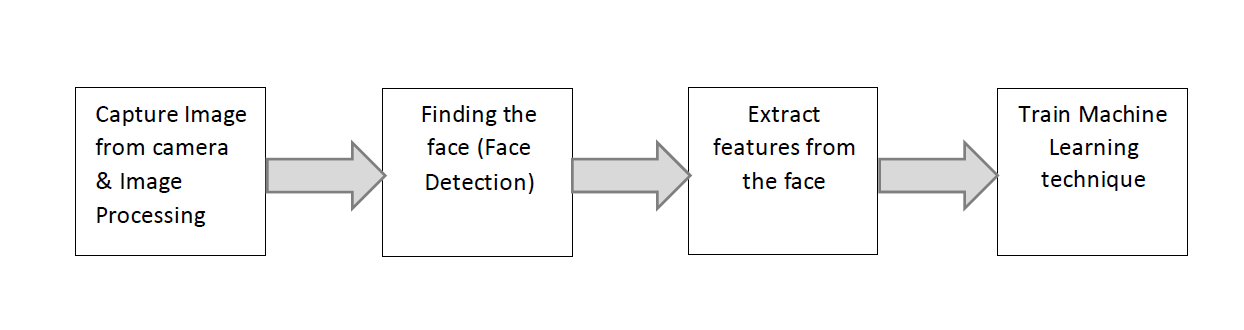
\includegraphics[scale=0.4]{4}
  \caption{The four stages for facial expression recognition}
  \label{fig:process}
\end{figure}
The related work looks at all four stages in the implementation process and different methods used by other researchers. The rest of this chapter is organised as follows: Section 2.1 describes the process of obtaining the image from the camera and image processing; Section 2.2 explains how face detection functions; Section 2.3 explains the feature extraction process; Section 2.4 the training of the machine learning technique and Section 2.5 outlines the results achived by other researchers.
%---------------------------------------------------------------
\section{Capture Image from the Camera and Image Processing}
An image is taken from the camera and image processing tools are used to help normalize and standardize the input image.
\begin{itemize}

\item Goyal and Mittal, achieved the desired resolution and colour for their images by adjusting the brightness and contrast of the image\cite{1}.

\item Reddy and Srinivas, scaled and cropped their images to \textit{(150X120)}, and ensured that the location of the eyes stayed the same in each image. The image was processed further, using an average combination of all the input image histograms. This process is called histogram equalization, see Figure~\ref{fig:hist eq}, and helps in decreasing variation in an image. Histogram equalization is a technique for stretching out the intensity range of an image to enhance the contrast of the image\cite{2}.

\begin{figure}[ht]
  \centering
  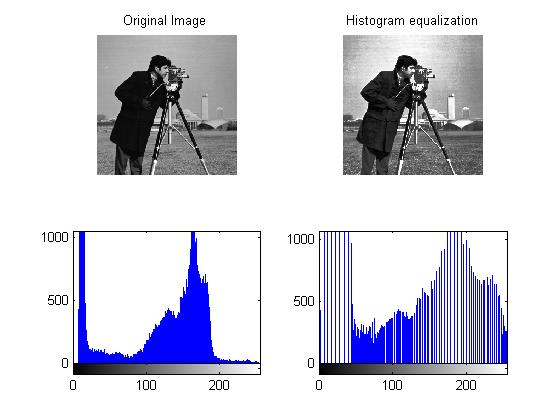
\includegraphics[scale=0.4]{5}
  \caption{Histogram Equalization}
  \label{fig:hist eq}
\end{figure}

\item Boubenna and Lee, scaled their images to \textit{(100X100)} pixels\cite{3}.

\end{itemize}
%---------------------------------------------------------------
\section{Face Detection - Finding the Face  }

Finding the location of the face helps identify the region that contains all the features required to continue with facial expression recognition. The rest of the image is not important for this purpose.
\begin{itemize}
\item Reddy and Srinivas applied a fixed oval shaped mask over the image to extract the face region\cite{2}. The images they used only contained faces, making it easier to apply the masks.

\begin{figure}[ht]
  \centering
  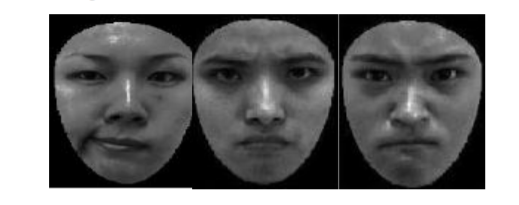
\includegraphics[scale=0.4]{6}
  \caption{Preprocessed Image with Oval Masks}
\end{figure}

\item Boubenna and Lee used the Viola and Jones algorithm to detect the location of the face in an image\cite{viola}. This algorithm uses Haar-like features to help find the facial features, such as the eyes, nose and mouth. The Ada Boost algorithm is used to reduce the number of features, if there are too many. They used the canny edge detection operator to detect the edges of the face\cite{3}.
\end{itemize}

%---------------------------------------------------------------

\section{Feature Extraction - Extract the Features from the Face }
Once the face has been detected, it is important to identify which features will be used for feature extraction. Either the full-face, or individual features from the face can be used as part of the feature set. These individual features can be the eyes, nose, mouth and eyebrows. The feature extraction algorithm can be applied based on its compatibility with the features chosen. 
\begin{itemize}
\item\ Goyal and Mittal extracted the nose, mouth and eyes using the Viola and Jones Haar classifier\cite{1}.

\item Reddy and Srinivas considered the entire face for the feature extraction not just the eyes, mouth and nose individually . First, they used Gabor filters to generate a bank of filters at 5 spatially varying frequencies and 8 orientations. The filtered outputs were then concatenated. Principle Component Analysis(PCA) was used to reduce dimensionality. PCA is a statistical technique that reduces the dimensions of feature vectors. The high dimensionality of feature vectors can cause over-fitting during classification. The PCA algorithm generates the eigenfaces for each image of dimension\textit{(NXN)}. From this their system generated the eigenvector of dimension \textit{(N2)} for each image. The vectors that relay the distribution of the face images the best are selected. These vectors are used to define the subspace(“face space”) of the face images\cite{2}. The face image subspace represents a lower dimentional space\textit{(N2)} of the original image with dimentions\textit{(NXN)}.

\item Boubenna and Lee used Pyramid Histogram of Oriented Gradients(PHOG) to extract features. PHOG represents an image by its local shape and the spatial layout. The local shape of an image is represented by a histogram of edge orientations within an image sub-region, which are divided into K bins. The spatial layout is represented by tiling the image into regions at different levels. Each image is divided into a sequence of increasingly finer spatial grids by repeatedly doubling the number of divisions in each axis direction\cite{phog}. The parameters of PHOG were set as follows: 3 for number of levels, 360 degrees for the number of dimentions and 16 for the number of bins. To decrease the number of features, a Genetic Algorithm(GA) was used, which resembles natural selection to find optimal features\cite{3}.
\end{itemize}

%---------------------------------------------------------------

\section{Training the machine learning technique}
The training of the machine learning technique based on supervised learning whereby the machine learning technique is given labelled images (Happy, Sad, Anger, Disgust, Surprise, Fear and Neutral) and is required to learn them. Once the machine learning technique has completed its training, it can then be fed unlabelled images, and the result would be a prediction of which label best suits the given image. 
\begin{itemize}
\item Goyal and Mittal used an Artificial Neural Network, with one hidden layer. The neural network architecture has three layers: input, hidden and output layers. Figure ~\ref{fig:nn} provides a visual layout of the architecture of an individual neuron and a ANN with multiple layers. Feed-forward ANNs allows the signal to travel in one direction from the input layer to the output layer. Recurrent networks contain feedback connections, where the signal moves in both directions. To get accurate results from the ANN, the weights can be set explicitly using prior knowledge, or the ANN can be trained to help find the optimal weights\cite{1, ann}.
\begin{figure}[ht]
  \centering
  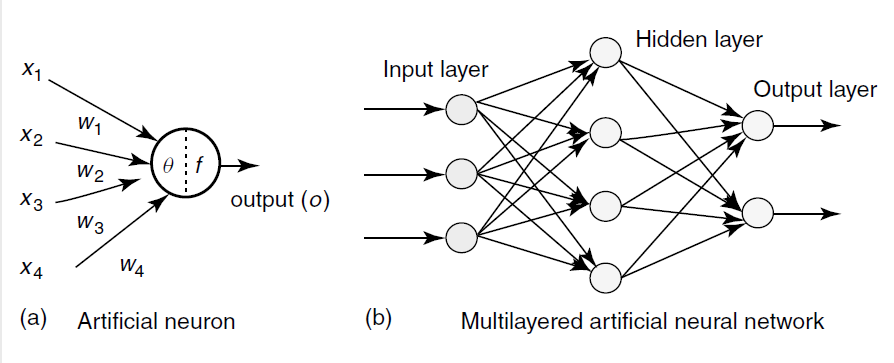
\includegraphics[scale=0.4]{8}
  \caption{Architecture of an artificial neuron and a multilayered neural network }
  \label{fig:nn}
\end{figure}
\item Reddy and Srinivas, used an Artificial Neural Network, with two hidden layers\cite{2}. 
\item Boubenna and Lee, used Linear Discriminants Analysis(LDA) and K Nearest Neighbours(KNN). LDA finds the maximum distances within classes, to obtain maximum class separation. LDA only uses up to second order moments, such as the covariance and mean, of the class distribution. KNN classifies unlabelled samples according to the training samples. KNN finds the nearest K in the labelled samples and set them to the closest group, for the unlabelled samples. One distance measure is required, and \cite{3} used the cosine distance measure.
\end{itemize}
%---------------------------------------------------------------
\section{Results}
The results from the three studies are as follows, with \cite{3} having the best overall results for their facial expression recognition system.
\begin{itemize}
\item Goyal and Mittal achieved an 80\% classification accuracy, using a confusion matrix and a regression plot to verify the results\cite{1}.
\item Reddy and Srinivas achieved an 85.7\% classification accuracy using the JAFFE database\cite{2}.
\item Boubenna and Lee achieved a 99.33\% accuracy, using the Radboud Faces Database(RaFD)\cite{3}.
\end{itemize}



\chapter{Image Processing Techniques} % Chapter 3
%

%\nocite{*}

\section{Introduction} % a.
This chapter looks at image processing techniques used in obtaining the features needed to do the final classification. The Viola and Jones algorithm, developed by Viola and Jones, is used to detect the location of the frontal face in the image. Once we have this location we then extract the face, which represents our region of interest. The region of interest is then Gray-scaled and is now ready for feature extraction. The Histogram of Oriented Gradients(HOG) is used for the feature extraction process. 

The rest of this chapter is organised as follows: Section 3.2 provides details on Viola-Jones Object Detection and it's key concepts; Section 3.3 covers the image pre-processing techniques used and Section 3.4 explains how Histogram of Oriented Gradients are used for feature extraction.

\section{Viola-Jones Object Detection}
\begin{flushleft}
The Viola-Jones algorithm \citep{viola} is an object detection method that uses Haar-like features. For this project the Viola-Jones object detection is used to find the location of frontal faces in images. The algorithm uses three concepts to effectively detect objects with certain features:\\

The first concept is the integral image, which allows for the features in the image to be evaluated much faster. This is also known as an intermediate view of the image. At each point$(x,y)$ in the integral image, there is the sum of the pixels above and to the left of the point$(x,y)$,inclusive.\\
Referring to Figure ~\ref{fig: integral}:
In order to calculate the sum of the pixels within the rectangle D, only four original  image references are needed.

\begin{itemize}
\item At point 1 in the integral image, the sum of all the pixels in rectangle A in the original image are used. 
\item At point 2 in the integral image the sum of all the pixels in rectangles A and B in the original image are added together(A+B). 
\item At point 3 in the integral image the sum of all the pixels in rectangles A and C in the original image are added together(A+C). 
\item Lastly, at point 4 in the integral image of all the rectangles are added together (A+B+C+D)in the original image. 
\end{itemize}
Thus, to get the sum of the pixels in rectangle D will result in 4+1-(2+3).
\end{flushleft}
\begin{figure}[H]
  \centering
  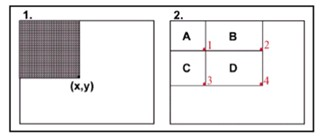
\includegraphics[scale=0.8]{1}
  \caption{Integral Image\citep{viola}}
  \label{fig: integral}
\end{figure}
\begin{flushleft}
The second concept in the Viola-Jones framework\citep{viola} is a classifier based on reducing a large feature set down to a smaller set of important features. This is done by using Ada-Boost. Ada-Boost finds a weak classifier and forces it to depend on a single feature, resulting in a stronger classifier. A weak classifier is selected at each stage of the boosting process, or feature selection process.

The third concept is a method that combines weak classifiers in a rejection cascade. This increases the speed of detection as the focus is now on promising areas of the image. Each stage in the cascade is formed using Ada-Boost. The Viola-Jones algorithm uses many Haar-like features. I will describe Three of these Haar-like features.
\begin{itemize}
  \item Two-rectangle feature - is calculated by subtracting the sum of the pixels of one rectangle from the sum of the other. The rectangles need to be the same size, shape and need to be vertically or horizontally adjacent.
  \item Three-rectangle feature - is calculated by subtracting the sum of the two outside rectangles from the middle rectangle.
  \item Four-rectangle feature - is calculated by subtracting the sum of the pixels of one diagonal pair from the other.
\end{itemize} 
\end{flushleft}
\begin{figure}[H]
  \centering
  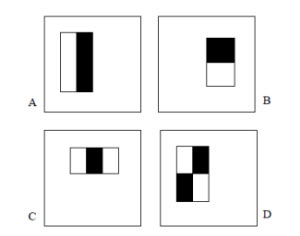
\includegraphics[scale=0.8]{2}
  \caption{Haar-like features\citep{viola}}
\end{figure}

\section{Image Preprocessing}
	\subsection{Resizing} 
	The image is resized once we obtain our region of interest using Viola-Jones to detect the location of the face. The main benefit of resizing the image is to maintain uniformity in our feature set. Another benefit is that it scales down the number of pixels in a image, resulting in a smaller feature set\cite{pre}. 
	\subsection{Gray Scaling}
	Converting an image from RGB(colour) to Grayscale helps in reducing the number of colour channels down to a single color channel. A commonly used method is the standard NTSC conversion formula, that calculates the luminance of a pixel\cite{pre}:

	Luminance of a pixel $= (0.2989 \times red) + (0.5870 \times green) + (0.1140 \times blue) $
	 
\section{Histogram of Oriented Gradients}   
The Histogram of Oriented Gradients is a feature extraction method for images. Where a image is divided into cells, of $C_x \times C_y$ pixels, that form a grid over the image. Histograms are calculated for each of these cells based on the orientation of the gradients of the pixels in the cell. This is followed by the image further being divided into a grid, of $B_x \times B_y$ cells, which are called blocks. Each block is used to contrast-normalize the histograms(cells) present in the block. The dimensions of the final feature vector calculated by: 

$\textrm{total number of blocks} \times \textrm{number of cells in each block} \times \textrm{number of orientation bins}$
\begin{flushleft}
Further details of the Histogram of Oriented Gradients will be discussed following Dalal \& Triggs HOG feature extraction chain,see Figure ~\ref{fig:hhog}, excluding the linear SVM and classification\cite{hog}.
\end{flushleft}
\begin{figure}[H]
  \centering
  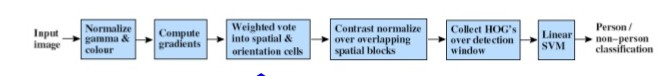
\includegraphics[scale=0.6]{chain}
  \caption{HOG feature extraction chain\cite{hog}}
  \label{fig:hhog}
\end{figure}

\subsection{Input Image}
Given an image, first identify the region of interest in the image. This region then forms your image window.
\begin{figure}[H]
\centering
\begin{minipage}{.5\textwidth}
  \centering
  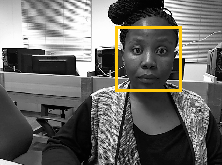
\includegraphics[width=.4\linewidth]{image}
  \captionof{figure}{Region of interest}
  \label{fig:test1}
\end{minipage}%
\begin{minipage}{.5\textwidth}
  \centering
  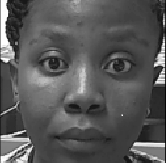
\includegraphics[width=.4\linewidth]{roi}
  \captionof{figure}{Image window}
  \label{fig:test2}
\end{minipage}
\end{figure}
\subsection{Normalize Gamma \& Colour}
Normalizing the image window is an optional addition to the HOG. Dalal \& Triggs found that normalizing the image pixels(p) at this the stage did not have a noticeable impact on the performance at the detection stage of their research.
However when choosing to normalize the image window Gamma (power law) normalization had a negative impact on the results, while Square-root normalization had more of a positive impact on the results.

Gamma Normalization: $log_(p)$ 

Square-root Normalization: $\sqrt{p}$
\subsection{Gradients}
The gradient for the image window is computed by applying a one dimensional mask in both X ($G_x$) and Y ($G_y$) directions.\

\begin{figure}[H]
  \centering
  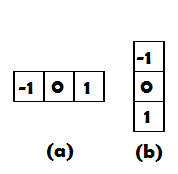
\includegraphics[scale=0.8]{sobel}
  \caption{One dimentional masks,(a)X-direction and (b) Y-direction}
\end{figure}
\begin{flushleft}
The mask convolves over the image window. At each point where the mask is placed the pixels are multiplied by the mask. After that the two outer pixels are added together and the result is placed in the position of the center pixel. The mask is not able to compute the gradients on the pixels around the egde of the image. Unless extra pixels are added to the edges of the image before hand. The example below shows how the loss in pixels affects the resulting gradient image.
\end{flushleft}
\subsubsection{Example:}

\begin{figure}[H]
\centering
\begin{subfigure}{.5\textwidth}
  \centering
  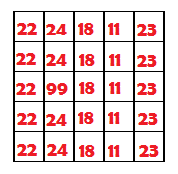
\includegraphics[width=.4\linewidth]{im}
  \label{fig:sub1}
\end{subfigure}%
\begin{subfigure}{.5\textwidth}
  \centering
  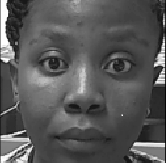
\includegraphics[width=.4\linewidth]{roi}
  \label{fig:sub2}
\end{subfigure}
\caption{Image window}
\label{fig:test}
\end{figure}
\begin{figure}[H]
\centering
\begin{subfigure}{.5\textwidth}
  \centering
  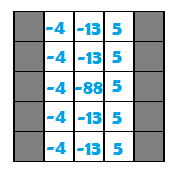
\includegraphics[width=.4\linewidth]{gx}
  \label{fig:sub1}
\end{subfigure}%
\begin{subfigure}{.5\textwidth}
  \centering
  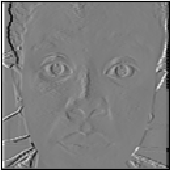
\includegraphics[width=.4\linewidth]{dx}
  \label{fig:sub2}
\end{subfigure}
\caption{The result of a one dimensional mask applied in the X-direction}
\label{fig:test}
\end{figure}
\begin{figure}[H]
\centering
\begin{subfigure}{.5\textwidth}
  \centering
  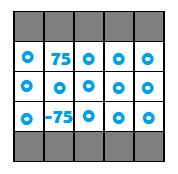
\includegraphics[width=.4\linewidth]{gy}
  \label{fig:sub1}
\end{subfigure}%
\begin{subfigure}{.5\textwidth}
  \centering
  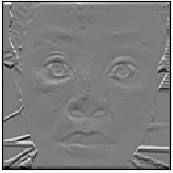
\includegraphics[width=.4\linewidth]{dy}
  \label{fig:sub2}
\end{subfigure}
\caption{The result of a one dimensional mask applied in the Y-direction}
\label{fig:test}
\end{figure}


Now that we have the gradients, we can compute the magnitude and orientation of the gradients from  $G_x$ \& $G_y$.

Magnitude: $G = \sqrt{G_x + G_y}$

Orientation: $\theta = arctan(\dfrac{G_y}{G_x})$

\subsection{Weighted Vote in Spatial \& Oriented Cells}
We can now decide on the dimensions of each cell, before calculating the HOGs. In their research Dalal \& Triggs found that the size of the cell are dependent on the size of the features you need to extract(e.g eyes, nose, mouth). 
\begin{figure}[H]
\centering
\begin{minipage}{.5\textwidth}
  \centering
  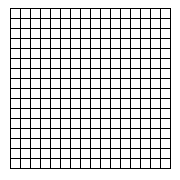
\includegraphics[width=.4\linewidth]{pixels}
  \captionof{figure}{$16 \times 16$ pixel image}
  \label{fig:test1}
\end{minipage}%
\begin{minipage}{.5\textwidth}
  \centering
  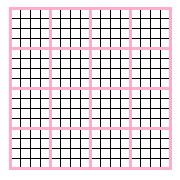
\includegraphics[width=.4\linewidth]{cells}
  \captionof{figure}{Image divided into $4 \times 4$ pixel cells}
  \label{fig:test2}
\end{minipage}
\end{figure}
The next parameter is the number of orientation bins. The orientation of the gradient can be described as the angle of the gradient. There are two options available when choosing the range of the gradient angle:
\begin{itemize}
  \item Signed [0,360] degrees
  \item Unsigned [0,180] degrees
\end{itemize}
Unsigned gradients in the range [0,180] degrees, with the number of orientation bins in the range [9,12] are the preferred values for the orientation bins.
\begin{figure}[H]
\centering
\begin{minipage}{.5\textwidth}
  \centering
  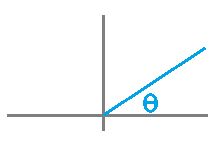
\includegraphics[width=.4\linewidth]{theta}
  \captionof{figure}{$\theta$ as an angle}
  \label{fig:test1}
\end{minipage}%
\begin{minipage}{.5\textwidth}
  \centering
  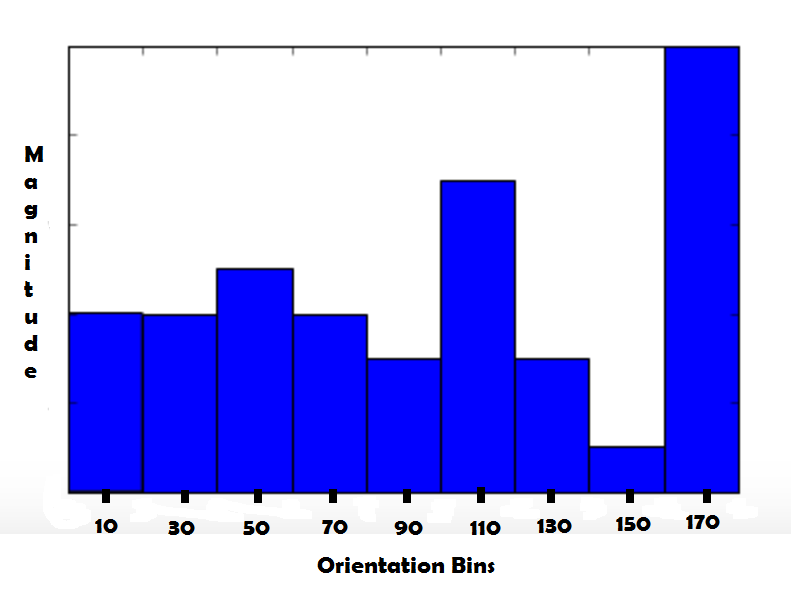
\includegraphics[width=.4\linewidth]{hist}
  \captionof{figure}{Unsigned gradients with 9 orientation bins}
  \label{fig:test2}
\end{minipage}
\end{figure}
Looking at a single cell. Each pixel of the gradient magnitude image contributes to a orientation bin of a cells histogram. The value of the same pixel in the gradient orientation image helps you identify which orientation bin to place the gradient magnitude of the pixel.

\subsection{Contrast Normalize over Overlapping spatial cells}
Contrast normalization is used to ensure that the cells are not affected vastly by changes illumination and contrast in the image. Starting with dividing the image into blocks that can fit at least 2-3 features, these blocks are allowed to overlap one another for more detailed feature set. Contrast normalization works by taking the sum of the histograms in a block $S_b$ and dividing each of the histograms $H_{hist}$ by $\sqrt{S_b ^2 + \epsilon ^2}$. The result is a normalized histogram $H_{norm}$ in each cell. 

Contrast normalization : $H_{norm} = \dfrac{H_{hist}}{\sqrt{S_b  ^2 + \epsilon ^2}}$
\begin{figure}[H]
\centering
\begin{minipage}{.5\textwidth}
  \centering
  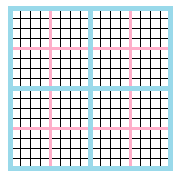
\includegraphics[width=.4\linewidth]{blocks}
  \captionof{figure}{Blocks of $B_x \times B_y$ cells}
  \label{fig:test1}
\end{minipage}%
\begin{minipage}{.5\textwidth}
  \centering
  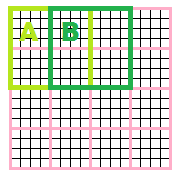
\includegraphics[width=.4\linewidth]{overlap}
  \captionof{figure}{Block A \& B with a 50\% overlap}
  \label{fig:test2}
\end{minipage}
\end{figure}

\begin{figure}[H]
  \centering
  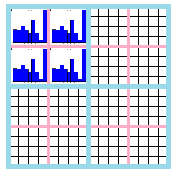
\includegraphics[scale=0.8]{norm}
  \caption{Cell histograms for contrast normalization in a block}
\end{figure}

\subsection{Collect HOGs over Detection Window}
The final step is to concatenate all the normalized histograms to form a one dimensional feature vector $[H_{norm}, H_{norm}, H_{norm}...]$. This feature vector is then used for the classification and training of the system.


\chapter{Implementation} % Chapter 2
%

%\nocite{*}

\section{Introduction} % a.
This chapter looks at the high-level and low-level views of the system and
code documentation. The high-level view in Section~\ref{sec:highlevel} provides an outline
of the processes followed during the implementation of the system, while
the low-level view in Section~\ref{sec:lowlevel} provides a more detailed description of
the implementation of the system.   

\section{High-Level View of the System}\label{sec:highlevel}
The high-level view of the system provides an overview of all the stages that the system follows when classifying an image given as input. These stages include: Capture Frame, Face Detection, Feature Extraction, Train Machine Learning Technique and Emotion Classification. Figure~\ref{fig: highlevel} serves as a visual aid for the content that follows.
\begin{figure}[H]
  \centering
  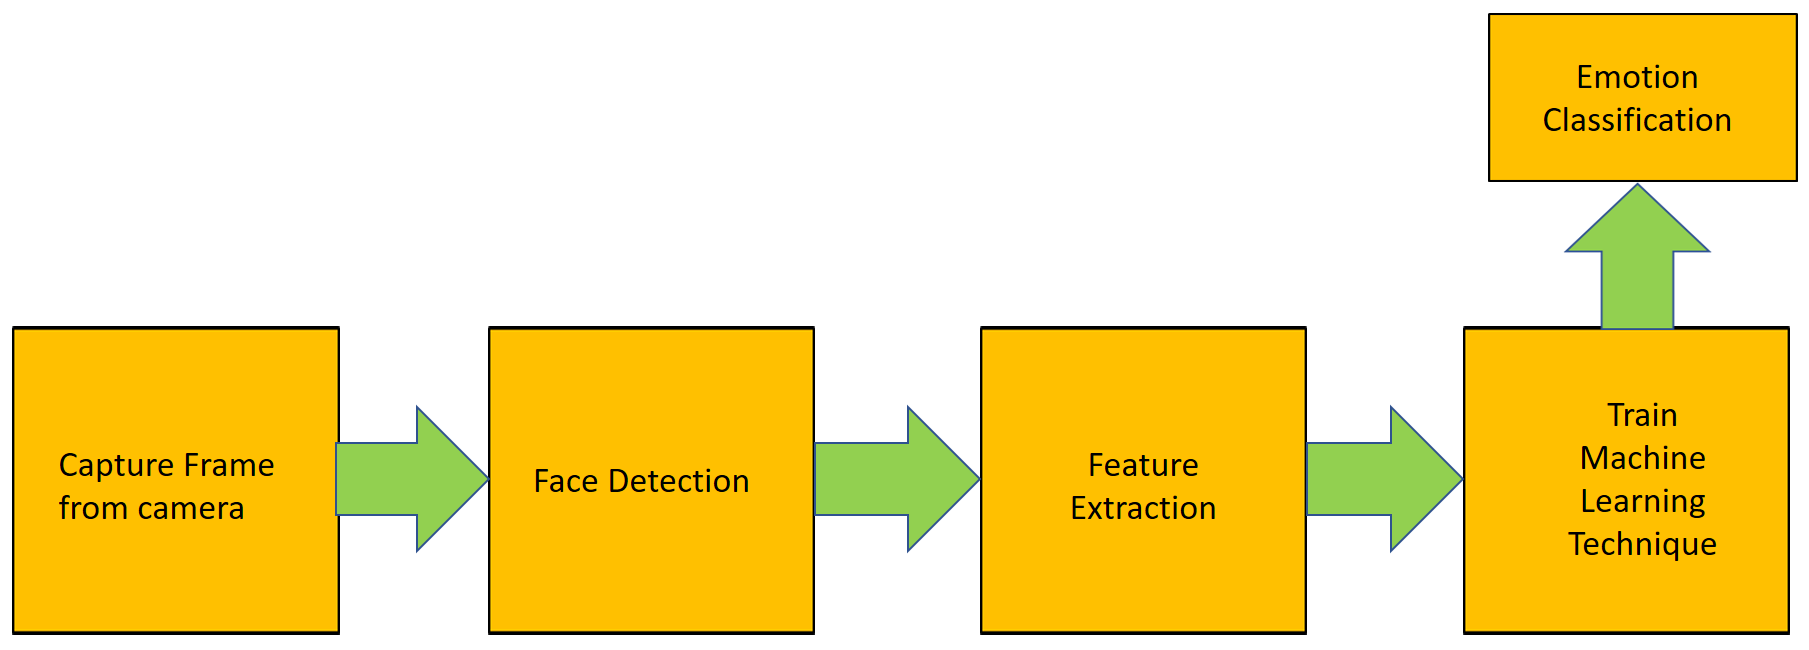
\includegraphics[scale=0.2]{pres1}
  \caption{High-Level View of System}
  \label{fig: highlevel}
\end{figure} 
Looking at Figure ~\ref{fig: highlevel}, the High-level view is explained as:

\begin{enumerate}
  \item \textbf{Capture Frame} -- The web camera records a constant stream of video input. The video input consists of a sequence of multiple image frames. The system captures each frame for processing as it is displayed on the video feed.

  \item \textbf{Face Detection} -- Now that we have captured a single frame, we need to check if there is a face present in the frame. This is done using a face detection algorithm. If a face is present in the frame, the location of the face is extracted. The rest of the image is disregarded at this point.

  \item \textbf{Feature Extraction} -- Every emotion displayed facially has it's own set of unique identifying features. By applying feature extraction we are able to represent these features in a way that a computer can understand and process. The feature extraction method is applied to the region of the image that contains the face.

  \item \textbf{Train Machine Learning Technique} -- Machine learning is a method used by computers to learn how to identify patterns in a given set of features. This process is called training. When we train the system, our features are labelled numerically from 1 to 7 and correspond with the classes (\textit{Angry, Disgust, Fear, Happy, Sadness, Surprise} and \textit{Neutral}). Labelling the features helps guide the computer in the learning process.

  \item \textbf{Emotion Classification} -- When the training is complete, classification helps to test the accuracy of the trained model. At this point the model should be able to identify emotions given unlabelled features.
\end{enumerate}

\clearpage
\section{Low-Level View of the System}\label{sec:lowlevel}
The high-level view of the system dives deeper into the details of the components used to implement the system. This is done following the same stages used in the high-level view of the system. In this section we will look at three conceptual low-level views that relate to our system. These views are aligned to the processes followed in image processing, Support Vector Machine model testing \& training and implementing the final system.
\subsection{Low-Level View of Image Processing}

The first low-level view is a visual representation of how the high-level view relates to the image processing techniques discussed in Chapter 3 is presented in Figure~\ref{fig: lowlevel}. 
\begin{figure}[H]
  \centering
  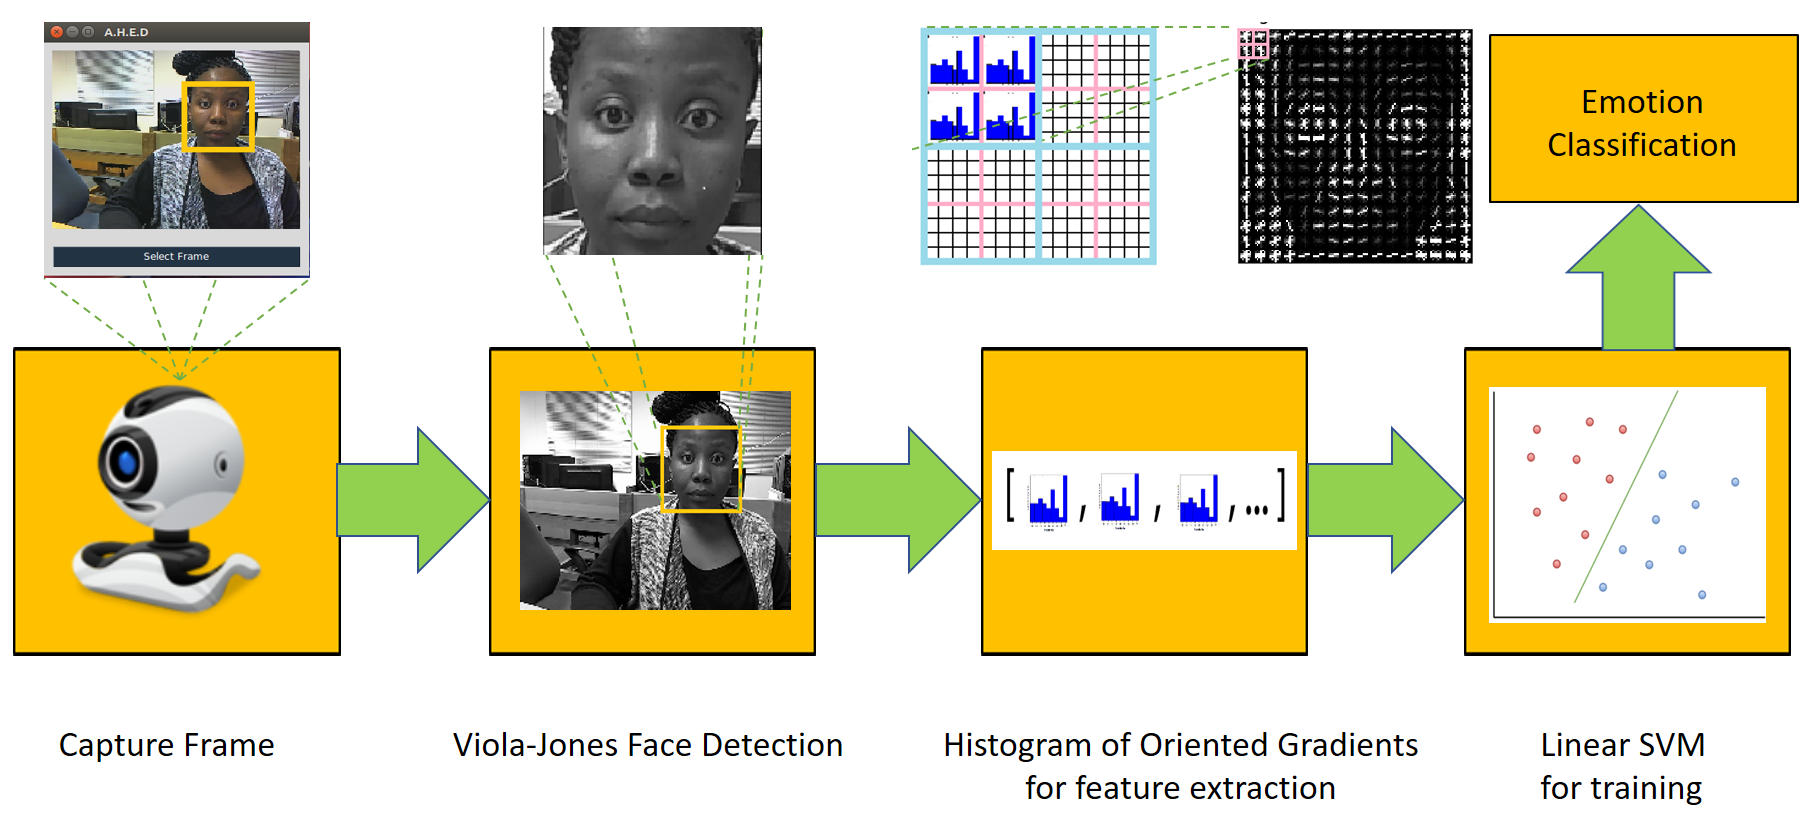
\includegraphics[scale=0.2]{pres2}
  \caption{Low-Level View of Image Processing}
  \label{fig: lowlevel}
\end{figure}


\subsection{Low-Level View of SVM Model Optimization, Testing \& Training}

The second low-level view relates to the training and testing of the SVM model used to classify the emotions. Where the `Capture Frame' stage is replaced by `Get Images from Dataset'. The results given in this section aim to contextualize the information given. The results pertaining to the testing or classification of the SVM model after training will be discussed further in Chapter 5. The code used to implement the SVM Optimization, Testing and Training can be found in Appendix B, Section B.1.2.
\begin{figure}[H]
  \centering
  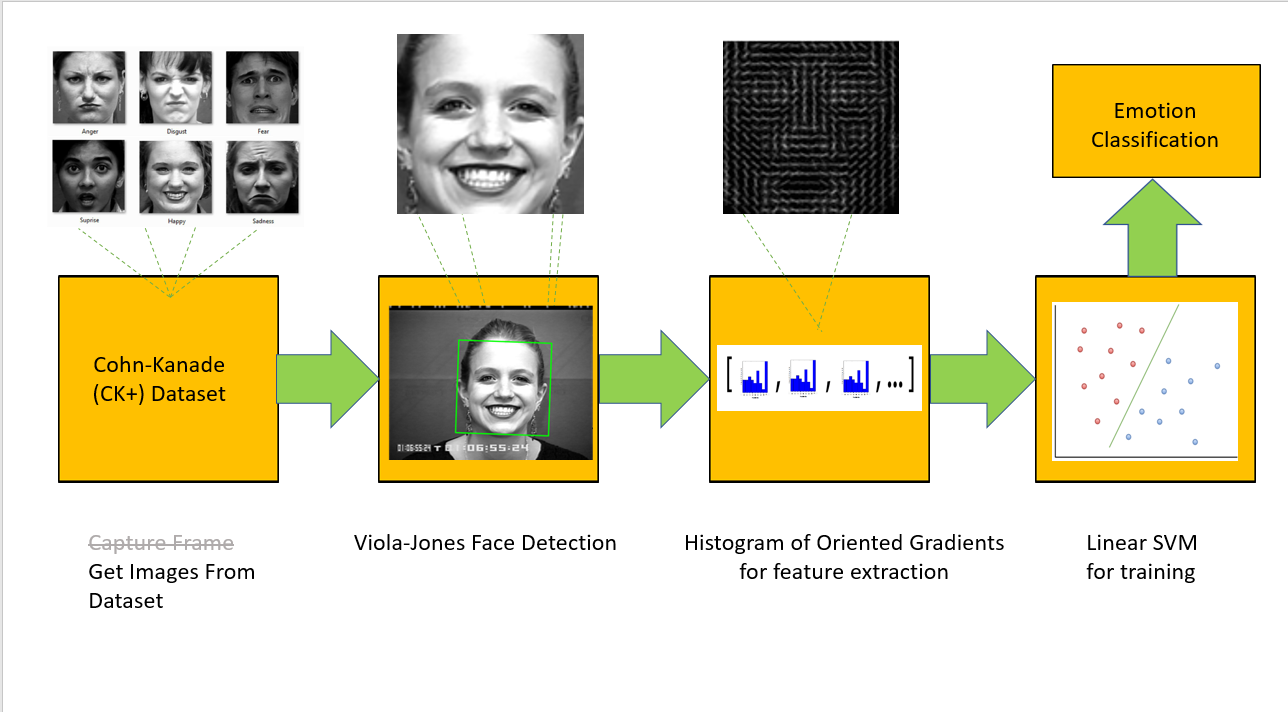
\includegraphics[scale=0.65]{second}
  \caption{Low-Level View of SVM Model Testing \& Training}
  \label{fig: lowlevel2}
\end{figure} 


Looking at Figure~\ref{fig: lowlevel2}, the Low-level view for SVM model testing and training is explained as:

\begin{enumerate}
  \item \textbf{Get Images From Dataset} -- The Extended Cohn-Kanade Dataset \citep{ck} is used as data for the training and testing of our SVM model. The images are divided into seven groups, whose labels are: \textit{Angry, Disgust, Fear, Happy, Sadness, Surprise} and \textit{Neutral}. The Table \ref{table:1} provides the total number of images present for each label.

\begin{table}[H]
\centering
\begin{tabular}{ |c||c|}	
	\hline
	\textbf{Emotion Label} & \textbf{N}  \\
	\hline 
	Angry & 45 \\ 
	Disgust & 59 \\ 
	Fear & 25 \\ 
	Happy & 69 \\ 
	Sadness & 28 \\ 
	Surprise & 83 \\  
	Neutral & 35 \\
	\hline  
\end{tabular}
\caption{CK+ Image Labels and Totals}
\label{table:1}
\end{table}

  \item \textbf{Face Detection} -- The Viola-Jones face detection is used to extract the face from each image in the CK+ dataset. The face region of the image is stored as a $56 \times 56$ pixel grayscale image. 
  
  \item \textbf{Feature Extraction} -- The resulting images from the face detection are used as inputs for the Histogram of Oriented Gradients which gives a one-dimensional feature vector for each image. Each image is given a numerical label from 1 to 7 based on the emotion displayed in the image, see Table \ref{table:22} for the labels. The feature vector is stored in the feature dataset with the corresponding numerical emotion label(e.g. [Numerical Label][Feature Vector]). 
\begin{table}[H]
\centering
\begin{tabular}{ |c||c|c|c|c|c|c|c|}
	\hline
	\textbf{Emotion Label}  & Angry & Disgust & Fear & Happy & Neutral & Sadness & Surprise \\ 
	\hline
	\textbf{Numerical Label} & 1 & 2 & 3 & 4 & 5 & 6 & 7   \\ 
	\hline
\end{tabular}   
\caption{Emotions with corresponding Labels for the feature vectors}
\label{table:22}
\end{table}

 The parameters used for the HOG are listed in Table \ref{table:2}. The optimization of the HOG parameters is discussed in Section 4.3.4.
\begin{table}[H]
\centering
\begin{tabular}{ |c|c|c|}
	\hline
	\textbf{Parameter} & \textbf{Size} & \textbf{Type}  \\
	\hline
	Image & $(56,56)$ & Pixels \\ 
	Cell & $(4,4)$ & Pixels \\ 
	Block & $(3,3)$ & Cells \\ 
	Overlap & $66.66 \%$ & Blocks \\ 
	Bins & $9$ & (0\si{\degree}-180\si{\degree}) Unsigned Gradients\\  
	\hline
	\multicolumn{3}{|c|}{Feature Vector Size: $11664$}\\ 
	\hline
\end{tabular}   
\caption{HOG Parameters}
\label{table:2}
\end{table}

  \item \textbf{Train Machine Learning Technique} -- The machine learning technique used to do the classification for our system is Support Vector Machines. \cite{ck} Used SVMs to test the accuracy of their CK+ dataset due to its proven accuracy with face and facial action detection. Binary classification is the simplest example for explaining how SVMs work. Where the SVM attempts to separate the closest negative and positive points in each class from each other. Once this separation is achieved it makes it easier to separate negative and positive points that are further away from each other, as the similarities in these points are less than those in the points that are closer. The distance between these points is calculated by subtracting the positive and negative points from each other. The positive and negative points closest to each other are considered our support vectors, these help in determining the separating hyperplane. The SVM needs to ensure that the distance between the support vectors is maximized. Figure~\ref{fig: svm} visualizes the concepts discussed.\\
  
  Considering that we have multiple classes in our dataset the `one versus all' method was used to train the SVM model. This is where one class is labelled as positive $(c)$ whilst the other classes are labelled as negative $(n-c)$. All of the classes $(n)$ are given the opportunity to be labelled as the positive class and the SVM model is generated.  

\begin{figure}[H]
  \centering
  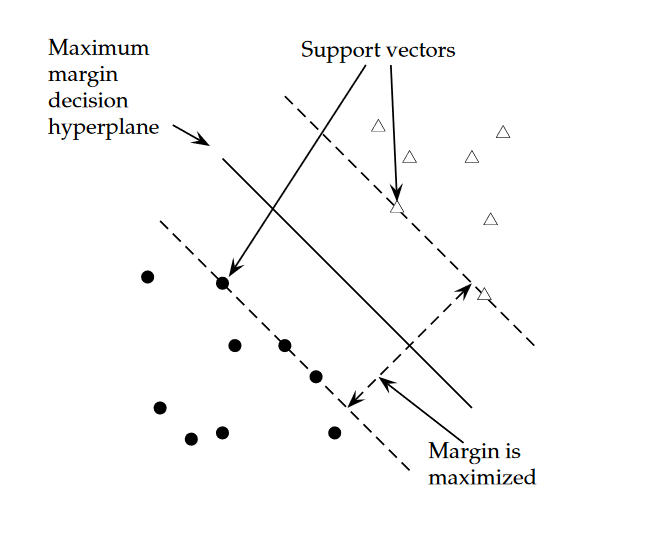
\includegraphics[scale=0.6]{svm}
  \caption{Key Functions of a SVM \cite{stan}}
  \label{fig: svm}
\end{figure} 





\begin{enumerate}
\item\textit{Cross-Validation} -- The feature dataset compiled after completing the feature extraction is used as input for the SVM. Where the dataset is divided into a training and testing dataset. The percentage of the split is dependent on how well the model performs with each split. A 60\% training and 40\% testing split was used for the SVM. Both these datasets should contain an equal distribution of the emotion labels in each dataset. This step ensures that all labels appear equally in both datasets. The Cross-validation score using a stratified K-fold of 3 is approximately 84\%. Cross-validation measures the overall performance of the SVM model on different training and testing data splits \cite{svm}. This tests the independence of the model to the dataset and helps to prevent overfitting in our model. K-fold cross-validation is done by splitting the dataset into K subsets of equal length. Each subset is then tested on the SVM model of the remaining K-1 subsets. Stratified K-fold cross-validation ensures that the classes are distributed equally in each subset. The training dataset is used as input for training our SVM and creating the SVM model that will be used in our system.\\

\item\textit{Grid-Search} -- After optimizing the SVM model with grid-search a Linear Kernel with a C of 1 was used. Grid search helps to find the optimal parameters for the SVM model. Where C determines the extent to which the SVM model should avoid misclassification in the training \cite{svm}. Larger values of C decrease the margin of the hyperplane which aims to increase the accuracy of the training. A smaller value for C increases the margin of the hyperplane, but carries the downside of more misclassified training data points. In \cite{svm} it is recommended that the optimal range of  that should to be investigated in order to find the best value for $C$ is $C = 2^{-5}, 2^{-3}, ..., 2^{15}$. 
\end{enumerate}






\item \textbf{Emotion Classification} -- The testing dataset is used to asses the performance of the the trained SVM model on unseen data. Where the SVM model is given the testing dataset features without the corresponding labels. The results of the SVM model classification are then compared to the original labels to test the accuracy of the SVM model. The SVM model trained for our system has an overall accuracy score of 88.2\%.\\
%\begin{enumerate}

%\begin{figure}[H]
%\centering
%\begin{minipage}{.485\textwidth}
%  \centering
%  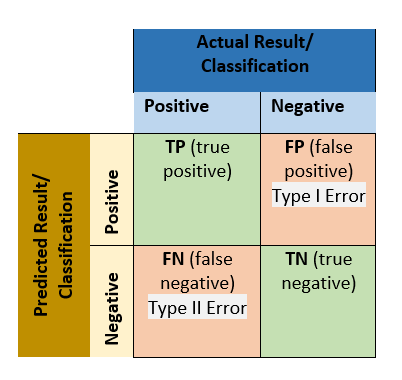
\includegraphics[width=.9\linewidth]{conf}
%  \captionof{figure}{Confusion Matrix}
%  \label{fig:conf}
%\end{minipage}%
%\begin{minipage}{.485\textwidth}
%  \centering
%  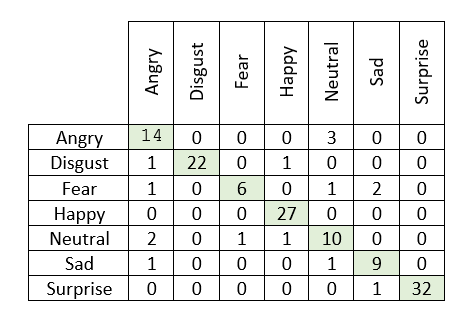
\includegraphics[width=.9\linewidth]{conf1}
%  \captionof{figure}{Confusion Matrix of SVM Model Classification}
%  \label{fig:conf1}
%\end{minipage}
%\end{figure}
%\end{enumerate}
 
\end{enumerate}

\subsection{Low-Level View of Final System}
The third low-level view shows how the process of Automatic Human Emotion Detection is streamlined for user interaction. Where classifications are performed live as the user changes their facial expressions. At this point we use the 'Trained SVM Model' with the HOG parameters from Table \ref{table:2} above.
\begin{figure}[H]
  \centering
  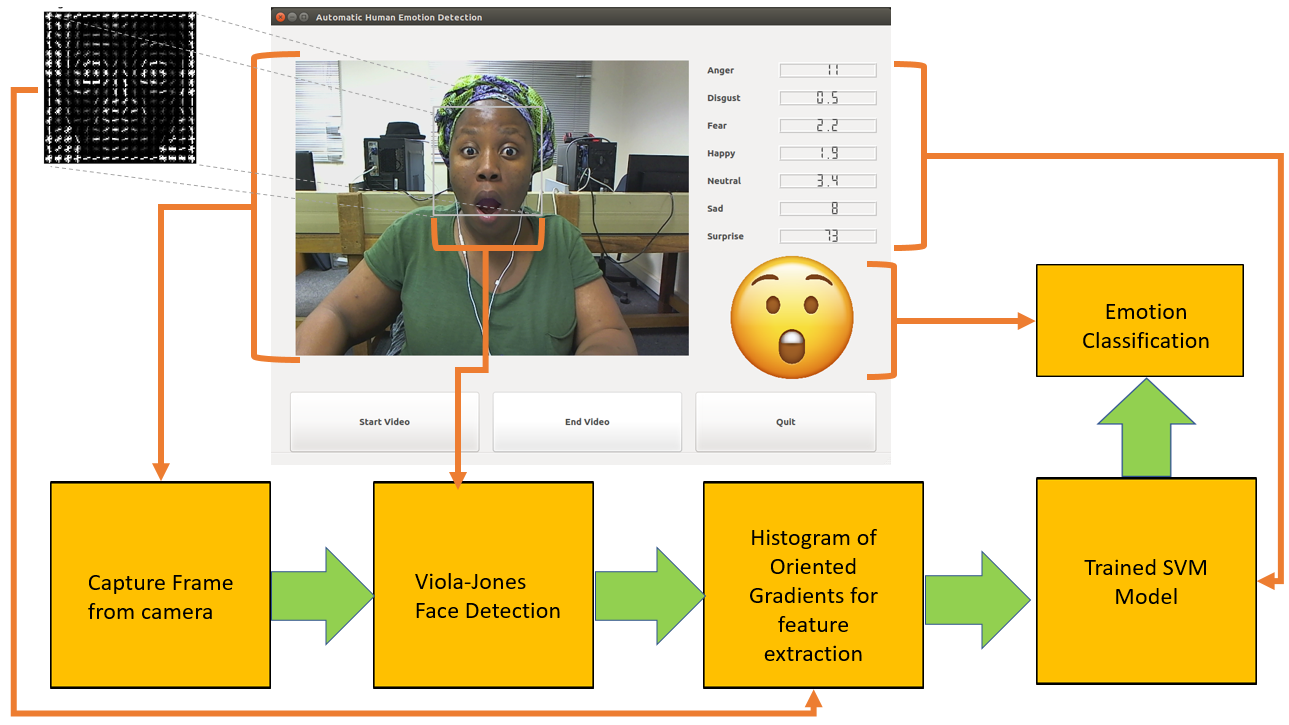
\includegraphics[scale=0.6]{demo}
  \caption{Low-Level View of Final System}
  \label{fig: lowlevel3}
\end{figure} 

\subsection{Optimizing HOG features}
This section covers the different combinations for the HOG parameters that were considered before the values in Table \ref{table:2} were chosen. The HOG implemented from scratch by us is compared to the OpenCV HOG using the Python Sklearn SVM library. All the other parameters remained the same at this point, the dataset had a 60\% training and 40\% testing dataset. The SVM model optimized to a Linear Kernel with a C of 1 for each iteration of the HOG features optimization. Both HOGs maintained a bin size of 9 and 50\% overlap for Block $(2,2)$, with a 66.66\% overlap for Block $(3,3)$.
\begin{table}[H]
\centering
\begin{tabular}{ |c||c|c|}
	\hline
	\multicolumn{3}{|c|}{\textbf{Accuracy of HOG Parameters}}\\
	\hline
	- & \textbf{Cell $(8,8)$ Block $(3,3)$} & \textbf{Cell $(4,4)$ Block $(3,3)$}\\
	\hline
	OpenCV HOG & 86\% & 88.2\% \\
	\hline
	AHED HOG & 77.9\% & 75.7\% \\
	\hline
	& \textbf{Cell $(8,8)$ Block $(2,2)$} & \textbf{Cell $(4,4)$ Block $(2,2)$}\\
	\hline
	OpenCV HOG & 83.8\% & 83.8\% \\
	\hline
	AHED HOG & 77.9\% & 82.3\% \\
	\hline
\end{tabular}
\caption{HOG Optimization}
\label{table:class}
\end{table}
\section{Conclusion}
The Automatic Human Emotion Detection system was implemented entirely using Python. OpenCV is used for the Viola-Jones face detection, Sklearn was used to implement the Histograms of Oriented gradients and the Support Vector Machines. The HOG implementation done from scratch used python numpy arrays and followed the implementation method discussed in Chapter 3. The highest accuracy achieved for the HOG implemented with OpenCV was 88.2\% and 82.3\% with the HOG implemented in this project. 




%\chapter{Testing} % Chapter 2
%


%\nocite{*}

\section{Introduction} % a.
This chapter looks at the results from training, testing and optimizing of the SVM Model selection process, in Section~\ref{sec:svm}. Table \ref{table: terms} gives an overview of the formulas and terms used in Figure ~\ref{fig:confu} and Table \ref{table:class} to describe the results.
\begin{table}[H]
\centering
\resizebox{\textwidth}{!}{
\begin{tabular}{ |c||c|c|}
	\hline
	\multicolumn{3}{|c|}{\textbf{SVM Model Evaluation}}\\
	\hline
      	\textbf{Term} &  \textbf{Formula} & \textbf{Description}\\
	\hline
      	\textbf{Type I Error} &      FP  &    False Positive   \\
	\hline
   	\textbf{Type II Error} &     FN  &    False Negative \\
	\hline
       	\textbf{Accuracy} &  $\frac{TP+TN}{TP+TN+FP+FN}$ & Evaluates the degree of correctness for the predictions   \\
	\hline
      	\textbf{Precision} &  $\frac{TP}{TP+FP}$ 	 &   The Positive predictive value \\
	\hline
    	\textbf{Recall} &     $\frac{TP}{TP+FP}$	 &   True positive rate  \\
	\hline
        \textbf{F1-Score} &  $2\times\frac{precision \times recall}{precision+recall}$  &   Evaluates the accuracy of predictions \\
	\hline
\end{tabular}}
\caption{Terminology and formulas used for evaluating the SVM Model \cite{dict}}
\label{table: terms}
\end{table}

%The testing of the entire system is followed in Section~\ref{sec:ahed}.

\subsection{Analysis of SVM Testing Results}\label{sec:svm}
The test set for testing the SVM model consisted of 136 entries, which is 40\% of the initial CK+ dataset. The overall accuracy of the SVM Model is 88.2\%, across all subjects and emotions. Table \ref{table:class} contains the `SVM Model Classification Report'. The report indicates the performance of each individual class, or emotion, and the overall estimated performance of the SVM model with regards to the precision, recall and f1-score. Classes that had more data available performed better overall as compared to those that had less. Since there was more testing data available for these classes. Working with an uneven dataset, see Figure~\ref{fig:pie}, makes it harder to judge the performance of each class in comparison to the other classes. \\
\begin{figure}[H]
  \centering
  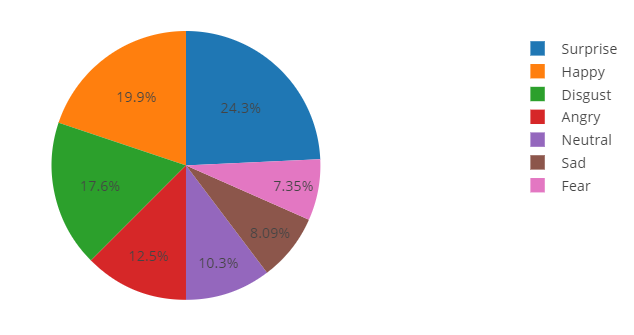
\includegraphics[scale=1.0]{pie}
  \caption{SVM test set breakdown}
  \label{fig:pie}
\end{figure}

The emotions labelled \textit{Disgust, Happy} and \textit{Surprise} had over 24 subjects in the test set. This resulted in a higher f1-score for prediction accuracy of these emotions. Where the emotions labelled \textit{Sad, Neutral, Fear} and \textit{Angry} had significantly lower f1-score and fewer subjects in the test set. 
\begin{table}[H]
\centering
\resizebox{\textwidth}{!}{
\begin{tabular}{ |c||c|c|c|c|}
	\hline
	\multicolumn{5}{|c|}{\textbf{SVM Model Classification Report}}\\
	\hline
      	\textbf{Label} &      \textbf{precision} &   \textbf{recall} & \textbf{f1-score} &  \textbf{Sample Total}\\
	\hline
      	\textbf{Angry} &      0.74  &    0.82  &    0.78  &      17\\
   	\textbf{Disgust} &      1.00  &    0.92  &    0.96  &      24\\
       	\textbf{Fear} &      0.86  &    0.60  &    0.71  &      10\\
      	\textbf{Happy} &      0.93  &    1.00  &    0.96  &      27\\
    	\textbf{Neutral} &      0.67  &    0.71  &    0.69  &      14\\
        \textbf{Sad} &      0.75  &    0.82  &    0.78  &      11 \\
   	\textbf{Surprise} &      1.00  &    0.97  &    0.98  &      33 \\
	\hline
	\textbf{Avg \/ Total}  &     0.89 &     0.88  &   0.88    &   136\\
	\hline
\end{tabular}}
\caption{SVM Classification Report}
\label{table:class}
\end{table}


\subsection{Analysis of Confusion Matrix for Test Results}


A confusion matrix summarises the outcomes of the classification based on the the actual labels of the testing data and those obtain from testing. The values obtained from the confusion matrix help with analyzing the SVM model. Figure~\ref{fig:confu} shows the confusion matrix for our SVM model. The diagonal starting at the top-left index till the bottom-right index contains all the true positives/negatives for our SVM model. Considering that a large portion of the test set lies on this diagonal, the model created is exceptionally stable and has a few random misclassifications. 

\begin{figure}[H]
  \centering
  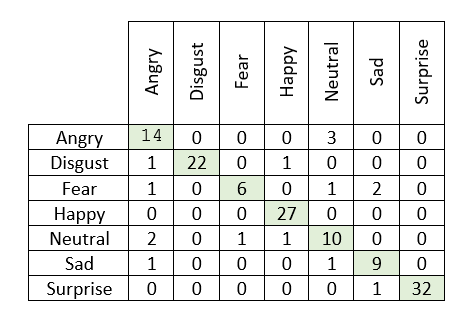
\includegraphics[scale=0.8]{conf1}
  \caption{Confusion Matrix of SVM Model Classification}
  \label{fig:confu}
\end{figure} 


\subsection{Analysis of SVM Testing Results for Subjects}
The results in the table,In Figure~\ref{fig: res1} and ~\ref{fig: res2}, look at all the individual subjects within the test set and their classification performance using the SVM model. The original CK+ dataset is uneven in that not all subjects had all seven emotions present in the dataset. This made it challenging to split the dataset evenly based on subjects. The split was done by ensuring that each emotion had the same test-train ratio for the training dataset and the testing dataset. 
\newline
\newline
In the results table, the green represents a correct classification under the indicated "Emotion Label" and the red blocks indicate a misclassification for that emotion and the misclassification is included in white text. Each subject had at least one emotion classified during testing, with a maximum of five emotions for subject 'S055'. 
The results in the table show that a vast majority of the blocks are shaded in green which indicates that most of the emotions were classified correctly, only a few of the blocks are shaded in red. None of the subjects had more than one misclassification, this indicates that the model is robust to changes in test subjects. See Figure~\ref{fig:faces} for a sample of the subjects in the CK+ dataset. The subjects are diverse in age, race and gender.

\begin{figure}[H]
  \centering
  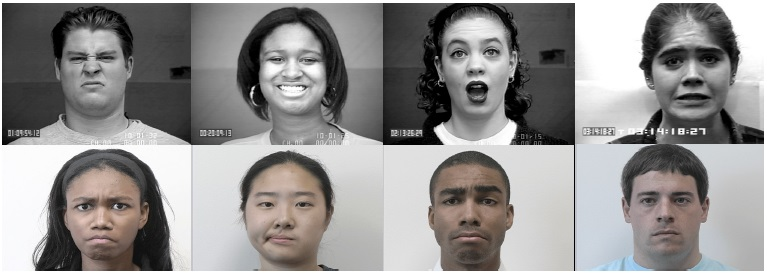
\includegraphics[scale=0.6]{faces}
  \caption{Subject sample from the CK+ Dataset \cite{ck}}
  \label{fig:faces}
\end{figure} 

\begin{figure}[H]
  \centering
  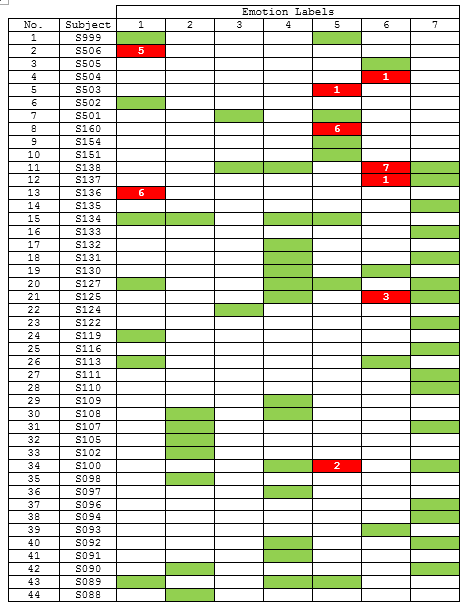
\includegraphics[scale=1.5]{res1}
  \caption{SVM Testing and Training Results for Subjects}
  \label{fig: res1}
\end{figure} 
\begin{figure}[H]
  \centering
  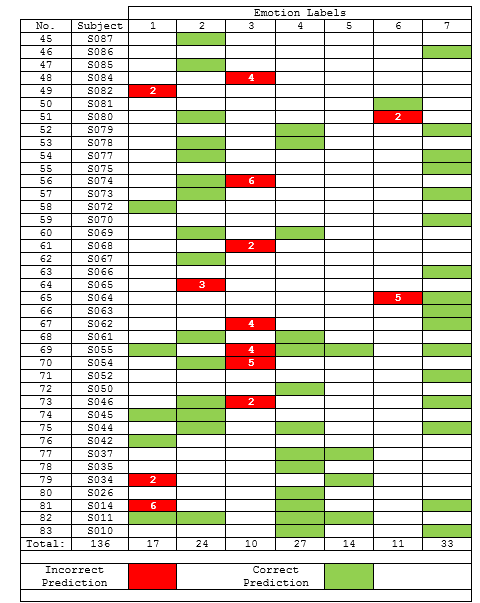
\includegraphics[scale=1.5]{res2}
  \caption{SVM Testing and Training Results for Subjects}
  \label{fig: res2}
\end{figure} 


\section{Conclusion}
The overall accuracy result for the SVM model was strong and generalized well with unseen data. Taking in to consideration that dataset used was not even, a further unbiased analysis on the results for individual subjects in the dataset was not possible. The dataset was split with the intention of having an equal ratio of subjects for each class in the testing set and the trainging set. As a result of this split analyzing the test results under each class proved to be more logical.

%\clearpage

%\subsection{Testing of AHED System}\label{sec:ahed}







%\chapter{User Guide} % Chapter 2
%

%\nocite{*}

\section{Introduction} % a.
This chapter covers all that is required from the users computer when running the AHED system. The AHED system has an interface for user interaction and provides live feedback on facial expressions. The interface is simple, see Figure~\ref{fig:gui}, and has the following funtionalities:
\begin{itemize}
\item A live video output stream. 
\item Real time emotion classification on the right hand side of the screen. This is where each emotion probability is given for the frame.
\item An Emoji(icon) that dispays the dominant emotion in the frame.
\item `Start Video' Button -- Initiates the video output stream.
\item `End Video' Button -- Pauses the video output stream.
\item `Quit' Button -- Closes the program window.
\end{itemize}
\begin{figure}[H]
  \centering
  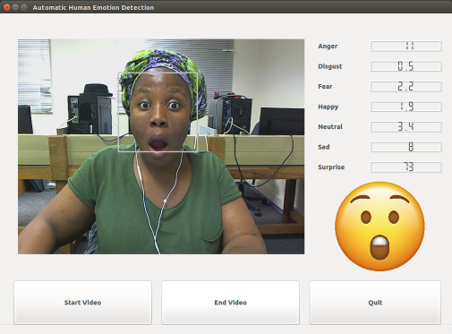
\includegraphics[scale= 0.8]{gui}
  \caption{The Graphical User Interface for the AHED System}
  \label{fig:gui}
\end{figure} 


\subsection{System Requirements}
These are the packages and programs needed to run the AHED system:
\begin{itemize}
\item Python 2.7
\item PyQt4
\item OpenCV
\item Webcamera (preferably HD 1080p)
\item Scikit-Image
\item Numpy
\item Pickle
\item Windows 10 or Ubuntu 16.04 operating sytem (preferably x64 and needs to support the libraries and packages above)
\item Note: Use JetBrains PyCharm on Windows, makes it easier to install missing libraries from python.
\end{itemize}

\subsection{Instructions}
Download `AHED.zip' from `http://cs.uwc.ac.za/~tlehata/index.html' under `Term 4'. After ensuring that your system requirements meet those stated above, unzip the `AHED.zip' folder. Open a terminal window or CMD window in the folder that contains `guiAHED.py'. To continue follow the instructions under your desired operating system.
\subsubsection{Ubuntu}
\begin{itemize} 
\item \$ workon cv
\item \$(cv) python guiAHED.py 
\end{itemize}
\subsubsection{Ubuntu}
\begin{itemize}
\item \$ python guiAHED.py 
\end{itemize}
A window should open up after a few seconds that looks the same as the one in Figure~\ref{fig:start}. After that you can proceed and press `Start Video' to start interacting with the system.
\begin{figure}[H]
  \centering
  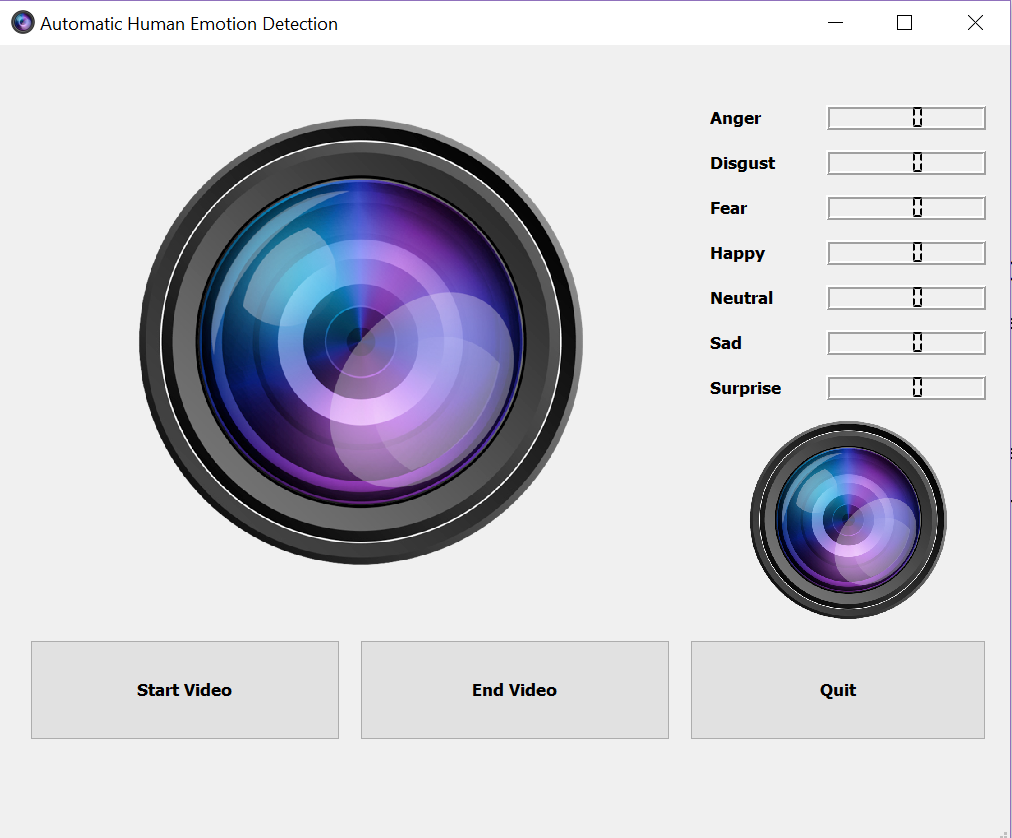
\includegraphics[scale=0.5]{start}
  \caption{Initial Start Interface for the AHED System}
  \label{fig:start}
\end{figure} 

\subsection{Feedback}
To leave feedback or for further assistance and questions send me an email on `3342317@myuwc.ac.za'.
%\chapter{Code Documentation} % Chapter 2
%

%\nocite{*}

\section{Introduction} % a.
This chapter includes all the source code used for implementing the Feature Extraction and SVM Training and Testing for the Automatic Human Emotion Detection system.
\subsection{Feature Extraction Python Code:}

    
%\begin{frame}[fragile]
 %      \begin{listing}[H]
%        \begin{pythoncode}    
\begin{lstlisting}{language=python}    
import sys
import cv2
import numpy as np
from skimage.feature import hog
from skimage import img_as_float

# a trained model for locating faces within an image
faceCascade = cv2.CascadeClassifier('Files/haarcascade_frontalface_alt.xml')

class FeatureExtraction():
    # ------------------------------------------------------------------------------
    # ----------------------------Viola-Jones Face Detection------------------------
    # ------------------------------------------------------------------------------
    def viola_jones(self, image):
        # set the height and width of face images
        height = 56
        width = 56
		
        # create an temporary 'image' of zeros
        scaled = np.zeros((height, width), dtype=np.float)
		
        # set the properties of the faceCascade
        faces = faceCascade.detectMultiScale(image, 1.3, 5)

        # set variables for finding the largest face in an image 
        max_size = 0  # w*h
        X = Y = W = H = 0
		
        # keeping track of x,y,w,h in order to find the biggest face
        for (x, y, w, h) in faces:  
            if max_size < w * h:
                max_size = w * h
                X = x
                Y = y
                W = w
                H = h
				
        # cater for when there are no faces in the image 'max_size = 0'
        if max_size != 0:
            # draw a rectangle identifying the location of the face in the image
            cv2.rectangle(image, (X, Y), (X + W, Y + H), (192, 192, 192), 2)
			
            # store the location with the face as our region of interest 'roi'
            roi = image[Y:Y + H, X:X + W]
			
            # convert the roi to grayscale
            gray = cv2.cvtColor(roi, cv2.COLOR_RGB2GRAY)
			
            # resize the roi so that all the roi's are uniform
            scaled = cv2.resize(gray, (height, width))

        return scaled, image

    # ------------------------------------------------------------------------------
    # -----------------------------------My HOG-------------------------------------
    # ------------------------------------------------------------------------------
    # Note: gradients work only on grayscale images

    # calculate the gradient in the X direction (gx)
    def gx(self, scaled):
        y, x = scaled.shape
        scaled = np.lib.pad(scaled, 1, 'constant', constant_values=0)
        gx = np.zeros((x, y))
        # sobelX:
        # [1	,0	,-1]
        # [2	,0	,-2]
        # [1	,0	,-1]
        for i in range(y):
            a = np.convolve(scaled[i - 1, :], [1, 0, -1], 'valid')
            b = np.convolve(scaled[i, :], [2, 0, -2], 'valid')
            c = np.convolve(scaled[i + 1, :], [1, 0, -1], 'valid')
            gx[i, :] = np.sum([a, b, c], axis=0)
        return gx
		
    # calculate the gradient in the Y direction (gy)
    def gy(self, scaled):
        y, x = scaled.shape
        scaled = np.lib.pad(scaled, 1, 'constant', constant_values=0)
        gy = np.zeros((x, y))
        # sobelY:
        # [-1	,-2	,-1]
        # [0	,0	,0]
        # [1	,2	,1]
        for j in range(x):
            a = np.convolve(scaled[:, j - 1], [1, 0, -1], 'valid')
            b = np.convolve(scaled[:, j], [2, 0, -2], 'valid')
            c = np.convolve(scaled[:, j + 1], [1, 0, -1], 'valid')
            gy[:, j] = np.sum([a, b, c], axis=0)
        return gy

    # calculate magnitude of the gradient('intensity')
    def magnitude(self, gx, gy):
        magnitude = np.sqrt(gx ** 2 + gy ** 2)
        return magnitude

    # calculate orientation of the gradient('direction')
    def orientation(self, gx, gy):
        # output is the same output as cv2.cartToPolar
        orientation = (np.arctan2(gy, gx) / np.pi) % 2 * np.pi  
        return orientation
	
    # calculate the HOG using an algorithm developed from my documentation
    def calculate_myhog(self, scaled):
        # gradients gx and gy
        gx = self.gx(scaled)
        gy = self.gy(scaled)

        # magnitude and orientation
        magnitude = self.magnitude(gx, gy)
        orientation = self.orientation(gx, gy)

        # orientation bins
        bin_n = 9
        bins = np.int32(bin_n * orientation / (2 * np.pi))

        # magnitude and orientation cells within a block
        bin_blocks = []
        mag_blocks = []
        epsilon = sys.float_info.epsilon

        # size of block
        blocksize = 3 
		
        # size of cell
        cellsize = 4

        # store the height and width of the face image(roi)
        width = scaled.shape[0]
        height = scaled.shape[1]

        # create the parameters for the block slider
        y = ((height - (cellsize * blocksize)) / cellsize) + 1
        x = ((width - (cellsize * blocksize)) / cellsize) + 1

        # stores all the histograms in an image
        histograms = []
		
        # loops through each block in a image(i,j)
        # using a block "slider" to capture all posible blocks 
        for i in range(0, y, 1):  
            for j in range(0, x, 1):
                # magnitude and orientation cells within a block
                bin_block = bins[i * cellsize: i * cellsize + blocksize * cellsize,
                            j * cellsize: j * cellsize + blocksize * cellsize]
                mag_block = magnitude[i * cellsize: i * cellsize + blocksize * cellsize,
                            j * cellsize: j * cellsize + blocksize * cellsize]
							
                tempHists = []
                sumHists = np.zeros((9,))
				
                # loops through each cell in a block(m,n)
                # this ensures that all the histograms in each cell are calculated
                for m in range(0, blocksize * cellsize, cellsize): 
                    for n in range(0, blocksize * cellsize, cellsize):
					
                        # magnitude and orientation cells within a cell
                        cellBin = bin_block[m:m + cellsize, n:n + cellsize]
                        cellMag = mag_block[m:m + cellsize, n:n + cellsize]
						
                        # temporarily store the histograms
                        tempHists.append(np.bincount(cellBin.ravel(), 
                        cellMag.ravel(), bin_n))
						
                        # store the sum of the histograms within a block
                        # this will be used for block normalization
                        sumHists = np.sum([sumHists, np.bincount(cellBin.ravel(), 
                        cellMag.ravel(), bin_n)], axis=0)
						
                # sum up all the bins
                sumHists = np.sum(sumHists)
				
                # normalize all the cell histograms in the block
                for hist in tempHists:
                    histograms.append(np.divide(hist, np.sqrt(
                    np.add(np.square(sumHists), np.square(epsilon)))))

                # store the magnitude and orientation for the block
                bin_blocks.append(bin_block)
                mag_blocks.append(mag_block)
        # create the HOG feature vector
        hist = np.hstack(histograms)
        return hist

    # ------------------------------------------------------------------------------
    # ---------------------------------OpenCV HOG-----------------------------------
    # ------------------------------------------------------------------------------
	
    # HOG implementation from skimage, using prefered parameters
    def hog_opencv(self, image):
        image = img_as_float(image)  # convert unit8 tofloat64 ... dtype
        orientations = 9		# orientation bins
        cellSize = (4, 4)		# pixels_per_cell
        blockSize = (3, 3)		# cells_per_block
        blockNorm = 'L1-sqrt'	# {'L1', 'L1-sqrt', 'L2', 'L2-Hys'}
        visualize = True		# Also return an image of the HOG.
        transformSqrt = False
        featureVector = True
        fd, hog_image = hog(image, orientations, cellSize, 
        blockSize, blockNorm, visualize, transformSqrt,
                            featureVector)
        return fd
		
    # testing features 
    def main(self):
        image = cv2.imread('Files/lense.png')
		scaled, image = self.viola_jones(image)
        print(self.calculate_myhog(scaled).shape)
		fd = self.hog_opencv(scaled)
		print(fd.shape)


if __name__ == '__main__': FeatureExtraction().main()
\end{lstlisting}%       \end{pythoncode}
%        \caption{Viola Jones Face Detection and HOG Feature Extraction, including self implemented HOG}
%    \end{listing}
%\end{frame}

 \clearpage
\subsection{SVM Training and Testing Python Code:}
%\begin{frame}[fragile]
      %\begin{listing}[H]
%        \begin{pythoncode}
\begin{lstlisting}{language=python}    
import sys
import pandas as pd
from sklearn import svm
from sklearn.model_selection import GridSearchCV, cross_val_score, StratifiedKFold, 
     train_test_split
from sklearn.metrics import confusion_matrix, accuracy_score, classification_report
import pickle


class Tester():
    def run_test(self, data, modelname):
        print '\n######################################################################'
        print '##########################~', modelname, '~#####################'
        print '######################################################################'

        dataset = pd.read_csv(data)

        X = dataset.ix[:, 1:].values
        y = dataset.ix[:, 0].values

        X_train, X_test, y_train, y_test = train_test_split(X, y, 
        test_size=.40, stratify=y, random_state=40)

        # Grid search parameters:
		
        # C = np.logspace(-5, 15,num=21,base = 2.0)
        # gamma = np.logspace(-15, 3, num=19,base = 2.0)
        param_grid = [
            {'C': [1, 10, 100, 1000], 'kernel': ['linear']},
            {'C': [1, 10, 100, 1000], 'gamma': [0.001, 0.0001], 'kernel': ['rbf']},
        ]
		
		# choose svm type: SVC - Support Vector Classification(based on libsvm)
        svc = svm.SVC(probability=True)

        print '\n######################################################################'
        print '#############################~SVM Grid Search~########################'
        print '######################################################################'
        clf = GridSearchCV(svc, param_grid)
        print '\t Parameter Grid:\n', param_grid

        print '\n######################################################################'
        print '##########################~SVM Cross Validation~######################'
        print '######################################################################'
        skf = StratifiedKFold(n_splits=3, random_state=None, shuffle=False)
        scores = cross_val_score(clf, X, y, cv=skf, n_jobs=-1)
        print '\t Cross validation scores: \t', scores
        print '\t Cross validation Accuracy:
        		\t %0.2f (+/- %0.2f)' % (scores.mean(), scores.std() * 2)

        print '\n######################################################################'
        print '#############################~SVM Train~##############################'
        print '######################################################################'
        clf = clf.fit(X_train, y_train)
        filename = modelname
        pickle.dump(clf, open('Files/'+filename, 'wb'))
        print '\t Best score for classifier:\t', clf.best_score_
        print '\t Best C:\t', clf.best_estimator_.C
        print '\t Best Kernel:\t', clf.best_estimator_.kernel
        print '\t Best Gamma:\t', clf.best_estimator_.gamma
        print '\t SVM Best Estimator:\t', clf.best_estimator_
        print '\n\t SVM Grid Scores: \n', clf.cv_results_

        print '\n######################################################################'
        print '#############################~SVM Predict~############################'
        print '######################################################################'
        clf = pickle.load(open('Files/'+modelname, 'rb'))
        y_pred = clf.predict(X_test)
        print 'SVM Classification Report:'
        print classification_report(y_test, y_pred,
                                    target_names=['Angry','Disgust','Fear',
                                    'Happy','Neutral','Sad', 'Surprise'])
        print 'SVM Confusion Matrix:'

        print confusion_matrix(y_test, y_pred, labels = [1,2,3,4,5,6,7])
        print '\t SVM Accuracy Score:', accuracy_score(y_test,y_pred,normalize=True)
        print 'file:', data

        print '\n######################################################################'
        print '#############################~SVM Test Results~############################'
        print '######################################################################'
        for i in range(len(X_test_names)):
            print 'Subject:',X_test_names[i],'\t Label:',y_test[i],
            		'\t Prediction:',y_pred[i]

    def main(self):
        print 'Output is printed to Files/test.out'
        orig_stdout = sys.stdout
        output = open('Files/test.out', 'w+')
        sys.stdout = output
        self.run_test('Files/dataCsv.csv', 'finalized_model.sav')
        sys.stdout.close()
        sys.stdout = orig_stdout
        print 'Done ^_^'
if __name__ == '__main__': Tester().main()
\end{lstlisting}%       \end{pythoncode}
%        \caption{SVM Training, Testing and Model Selection \& Optimization}
%    \end{listing}
%\end{frame}

%\appendix
\renewcommand{\chaptermark}[1]%
	{\markboth{Appendix \thechapter. #1}{}}
\setcounter{chapter}{0}

\chapter{Title of Appendix A}
\label{appendixA}

\section{The pilot questionnaire}


\begin{figure}
This is a dummy figure and it should be numbered A.1.
\caption{This figure is in Appendix A and is numbered A.1}
\end{figure}

\begin{figure}
This is a dummy figure and it should be numbered A.2.
\caption{This figure is in Appendix A and is numbered A.2}
\end{figure}

\begin{table}
\caption{This is table A.1}
\begin{tabular}{ll}
nothing& nothing\\
nothing& nothing\\
\end{tabular}

\end{table}



%\appendix
\setcounter{chapter}{1}
\renewcommand{\chaptermark}[1]%
	{\markboth{Appendix \thechapter. #1}{}}
\chapter{Examples of index entries}
\label{appendixB}

\section{Introduction} % a.

``Several other terms have 
been coined previously for this rapidly advancing area, such as 
\emph{connectionist processing}\index{processing!connectionist} 
\citep{shas95}, 
\emph{parallel distributed processing}\index{parallel distributed
processing}\index{PDP}
(PDP) \citep{rume86},
\emph{artificial neural networks}\index{artificial neural
network}\index{ANN!see {network, neural network}}\index{artificial neural
network|see {ANN, network, neural network}}
(ANN)~\citep{hass95,roja96},
and 
\emph{artificial neural systems}\index{artificial neural system}
\citep{zurada92}.
This book assumes a basic familiarity with neurocomputing. However, 
those readers requiring more information should page to Chapter~13 
where an introduction is given.

In \emph{knowledge-based}  neurocomputing\index{knowledge-based!neurocomputing} the emphasis is on the use 
and representation of knowledge\index{knowledge} about an application within the 
neurocomputing paradigm.''\\

This is the end of the quotation.

``Several other terms have 
been coined previously for this rapidly advancing area, such as 
\emph{connectionist processing}\index{processing!connectionist} 
\citep{shas95}, 
\emph{parallel distributed processing}\index{parallel distributed
processing}\index{PDP}
(PDP) \citep{rume86},
\emph{artificial neural networks}\index{artificial neural
network}\index{ANN!see {network, neural network}}\index{artificial neural
network|see {ANN, network, neural network}}
(ANN)~\citep{hass95,roja96},
and 
\emph{artificial neural systems}\index{artificial neural system}
\citep{zurada92}.
This book assumes a basic familiarity with neurocomputing. However, 
those readers requiring more information should page to Chapter~13 
where an introduction is given.

In \emph{knowledge-based}  neurocomputing\index{knowledge-based!neurocomputing} the emphasis is on the use 
and representation of knowledge\index{knowledge} about an application within the 
neurocomputing paradigm.''\\

This is the end of the quotation.

``Several other terms have 
been coined previously for this rapidly advancing area, such as 
\emph{connectionist processing}\index{processing!connectionist} 
\citep{shas95}, 
\emph{parallel distributed processing}\index{parallel distributed
processing}\index{PDP}
(PDP) \citep{rume86},
\emph{artificial neural networks}\index{artificial neural
network}\index{ANN!see {network, neural network}}\index{artificial neural
network|see {ANN, network, neural network}}
(ANN)~\citep{hass95,roja96},
and 
\emph{artificial neural systems}\index{artificial neural system}
\citep{zurada92}.
This book assumes a basic familiarity with neurocomputing. However, 
those readers requiring more information should page to Chapter~13 
where an introduction is given.

In \emph{knowledge-based}  neurocomputing\index{knowledge-based!neurocomputing} the emphasis is on the use 
and representation of knowledge\index{knowledge} about an application within the 
neurocomputing paradigm.''\\

This is the end of the quotation.

``Several other terms have 
been coined previously for this rapidly advancing area, such as 
\emph{connectionist processing}\index{processing!connectionist} 
\citep{shas95}, 
\emph{parallel distributed processing}\index{parallel distributed
processing}\index{PDP}
(PDP) \citep{rume86},
\emph{artificial neural networks}\index{artificial neural
network}\index{ANN!see {network, neural network}}\index{artificial neural
network|see {ANN, network, neural network}}
(ANN)~\citep{hass95,roja96},
and 
\emph{artificial neural systems}\index{artificial neural system}
\citep{zurada92}.
This book assumes a basic familiarity with neurocomputing. However, 
those readers requiring more information should page to Chapter~13 
where an introduction is given.

In \emph{knowledge-based}  neurocomputing\index{knowledge-based!neurocomputing} the emphasis is on the use 
and representation of knowledge\index{knowledge} about an application within the 
neurocomputing paradigm.''\\

This is the end of the quotation.

``Several other terms have 
been coined previously for this rapidly advancing area, such as 
\emph{connectionist processing}\index{processing!connectionist} 
\citep{shas95}, 
\emph{parallel distributed processing}\index{parallel distributed
processing}\index{PDP}
(PDP) \citep{rume86},
\emph{artificial neural networks}\index{artificial neural
network}\index{ANN!see {network, neural network}}\index{artificial neural
network|see {ANN, network, neural network}}
(ANN)~\citep{hass95,roja96},
and 
\emph{artificial neural systems}\index{artificial neural system}
\citep{zurada92}.
This book assumes a basic familiarity with neurocomputing. However, 
those readers requiring more information should page to Chapter~13 
where an introduction is given.

In \emph{knowledge-based}  neurocomputing\index{knowledge-based!neurocomputing} the emphasis is on the use 
and representation of knowledge\index{knowledge} about an application within the 
neurocomputing paradigm.''\\

This is the end of the quotation.

``Several other terms have 
been coined previously for this rapidly advancing area, such as 
\emph{connectionist processing}\index{processing!connectionist} 
\citep{shas95}, 
\emph{parallel distributed processing}\index{parallel distributed
processing}\index{PDP}
(PDP) \citep{rume86},
\emph{artificial neural networks}\index{artificial neural
network}\index{ANN!see {network, neural network}}\index{artificial neural
network|see {ANN, network, neural network}}
(ANN)~\citep{hass95,roja96},
and 
\emph{artificial neural systems}\index{artificial neural system}
\citep{zurada92}.
This book assumes a basic familiarity with neurocomputing. However, 
those readers requiring more information should page to Chapter~13 
where an introduction is given.

In \emph{knowledge-based}  neurocomputing\index{knowledge-based!neurocomputing} the emphasis is on the use 
and representation of knowledge\index{knowledge} about an application within the 
neurocomputing paradigm.''\\

This is the end of the quotation.

``Several other terms have 
been coined previously for this rapidly advancing area, such as 
\emph{connectionist processing}\index{processing!connectionist} 
\citep{shas95}, 
\emph{parallel distributed processing}\index{parallel distributed
processing}\index{PDP}
(PDP) \citep{rume86},
\emph{artificial neural networks}\index{artificial neural
network}\index{ANN!see {network, neural network}}\index{artificial neural
network|see {ANN, network, neural network}}
(ANN)~\citep{hass95,roja96},
and 
\emph{artificial neural systems}\index{artificial neural system}
\citep{zurada92}.
This book assumes a basic familiarity with neurocomputing. However, 
those readers requiring more information should page to Chapter~13 
where an introduction is given.

In \emph{knowledge-based}  neurocomputing\index{knowledge-based!neurocomputing} the emphasis is on the use 
and representation of knowledge\index{knowledge} about an application within the 
neurocomputing paradigm.''\\

This is the end of the quotation.

``Several other terms have 
been coined previously for this rapidly advancing area, such as 
\emph{connectionist processing}\index{processing!connectionist} 
\citep{shas95}, 
\emph{parallel distributed processing}\index{parallel distributed
processing}\index{PDP}
(PDP) \citep{rume86},
\emph{artificial neural networks}\index{artificial neural
network}\index{ANN!see {network, neural network}}\index{artificial neural
network|see {ANN, network, neural network}}
(ANN)~\citep{hass95,roja96},
and 
\emph{artificial neural systems}\index{artificial neural system}
\citep{zurada92}.
This book assumes a basic familiarity with neurocomputing. However, 
those readers requiring more information should page to Chapter~13 
where an introduction is given.

In \emph{knowledge-based}  neurocomputing\index{knowledge-based!neurocomputing} the emphasis is on the use 
and representation of knowledge\index{knowledge} about an application within the 
neurocomputing paradigm.''\\

This is the end of the quotation.

``Several other terms have 
been coined previously for this rapidly advancing area, such as 
\emph{connectionist processing}\index{processing!connectionist} 
\citep{shas95}, 
\emph{parallel distributed processing}\index{parallel distributed
processing}\index{PDP}
(PDP) \citep{rume86},
\emph{artificial neural networks}\index{artificial neural
network}\index{ANN!see {network, neural network}}\index{artificial neural
network|see {ANN, network, neural network}}
(ANN)~\citep{hass95,roja96},
and 
\emph{artificial neural systems}\index{artificial neural system}
\citep{zurada92}.
This book assumes a basic familiarity with neurocomputing. However, 
those readers requiring more information should page to Chapter~13 
where an introduction is given.

In \emph{knowledge-based}  neurocomputing\index{knowledge-based!neurocomputing} the emphasis is on the use 
and representation of knowledge\index{knowledge} about an application within the 
neurocomputing paradigm.''\\

This is the end of the quotation.

``Several other terms have 
been coined previously for this rapidly advancing area, such as 
\emph{connectionist processing}\index{processing!connectionist} 
\citep{shas95}, 
\emph{parallel distributed processing}\index{parallel distributed
processing}\index{PDP}
(PDP) \citep{rume86},
\emph{artificial neural networks}\index{artificial neural
network}\index{ANN!see {network, neural network}}\index{artificial neural
network|see {ANN, network, neural network}}
(ANN)~\citep{hass95,roja96},
and 
\emph{artificial neural systems}\index{artificial neural system}
\citep{zurada92}.
This book assumes a basic familiarity with neurocomputing. However, 
those readers requiring more information should page to Chapter~13 
where an introduction is given.

In \emph{knowledge-based}  neurocomputing\index{knowledge-based!neurocomputing} the emphasis is on the use 
and representation of knowledge\index{knowledge} about an application within the 
neurocomputing paradigm.''\\

This is the end of the quotation.

``Several other terms have 
been coined previously for this rapidly advancing area, such as 
\emph{connectionist processing}\index{processing!connectionist} 
\citep{shas95}, 
\emph{parallel distributed processing}\index{parallel distributed
processing}\index{PDP}
(PDP) \citep{rume86},
\emph{artificial neural networks}\index{artificial neural
network}\index{ANN!see {network, neural network}}\index{artificial neural
network|see {ANN, network, neural network}}
(ANN)~\citep{hass95,roja96},
and 
\emph{artificial neural systems}\index{artificial neural system}
\citep{zurada92}.
This book assumes a basic familiarity with neurocomputing. However, 
those readers requiring more information should page to Chapter~13 
where an introduction is given.

In \emph{knowledge-based}  neurocomputing\index{knowledge-based!neurocomputing} the emphasis is on the use 
and representation of knowledge\index{knowledge} about an application within the 
neurocomputing paradigm.''\\

This is the end of the quotation.

``Several other terms have 
been coined previously for this rapidly advancing area, such as 
\emph{connectionist processing}\index{processing!connectionist} 
\citep{shas95}, 
\emph{parallel distributed processing}\index{parallel distributed
processing}\index{PDP}
(PDP) \citep{rume86},
\emph{artificial neural networks}\index{artificial neural
network}\index{ANN!see {network, neural network}}\index{artificial neural
network|see {ANN, network, neural network}}
(ANN)~\citep{hass95,roja96},
and 
\emph{artificial neural systems}\index{artificial neural system}
\citep{zurada92}.
This book assumes a basic familiarity with neurocomputing. However, 
those readers requiring more information should page to Chapter~13 
where an introduction is given.

In \emph{knowledge-based}  neurocomputing\index{knowledge-based!neurocomputing} the emphasis is on the use 
and representation of knowledge\index{knowledge} about an application within the 
neurocomputing paradigm.''\\

This is the end of the quotation.

``Several other terms have 
been coined previously for this rapidly advancing area, such as 
\emph{connectionist processing}\index{processing!connectionist} 
\citep{shas95}, 
\emph{parallel distributed processing}\index{parallel distributed
processing}\index{PDP}
(PDP) \citep{rume86},
\emph{artificial neural networks}\index{artificial neural
network}\index{ANN!see {network, neural network}}\index{artificial neural
network|see {ANN, network, neural network}}
(ANN)~\citep{hass95,roja96},
and 
\emph{artificial neural systems}\index{artificial neural system}
\citep{zurada92}.
This book assumes a basic familiarity with neurocomputing. However, 
those readers requiring more information should page to Chapter~13 
where an introduction is given.

In \emph{knowledge-based}  neurocomputing\index{knowledge-based!neurocomputing} the emphasis is on the use 
and representation of knowledge\index{knowledge} about an application within the 
neurocomputing paradigm.''\\

This is the end of the quotation.

``Several other terms have 
been coined previously for this rapidly advancing area, such as 
\emph{connectionist processing}\index{processing!connectionist} 
\citep{shas95}, 
\emph{parallel distributed processing}\index{parallel distributed
processing}\index{PDP}
(PDP) \citep{rume86},
\emph{artificial neural networks}\index{artificial neural
network}\index{ANN!see {network, neural network}}\index{artificial neural
network|see {ANN, network, neural network}}
(ANN)~\citep{hass95,roja96},
and 
\emph{artificial neural systems}\index{artificial neural system}
\citep{zurada92}.
This book assumes a basic familiarity with neurocomputing. However, 
those readers requiring more information should page to Chapter~13 
where an introduction is given.

In \emph{knowledge-based}  neurocomputing\index{knowledge-based!neurocomputing} the emphasis is on the use 
and representation of knowledge\index{knowledge} about an application within the 
neurocomputing paradigm.''\\

This is the end of the quotation.

``Several other terms have 
been coined previously for this rapidly advancing area, such as 
\emph{connectionist processing}\index{processing!connectionist} 
\citep{shas95}, 
\emph{parallel distributed processing}\index{parallel distributed
processing}\index{PDP}
(PDP) \citep{rume86},
\emph{artificial neural networks}\index{artificial neural
network}\index{ANN!see {network, neural network}}\index{artificial neural
network|see {ANN, network, neural network}}
(ANN)~\citep{hass95,roja96},
and 
\emph{artificial neural systems}\index{artificial neural system}
\citep{zurada92}.
This book assumes a basic familiarity with neurocomputing. However, 
those readers requiring more information should page to Chapter~13 
where an introduction is given.

In \emph{knowledge-based}  neurocomputing\index{knowledge-based!neurocomputing} the emphasis is on the use 
and representation of knowledge\index{knowledge} about an application within the 
neurocomputing paradigm.''\\

This is the end of the quotation.

``Several other terms have 
been coined previously for this rapidly advancing area, such as 
\emph{connectionist processing}\index{processing!connectionist} 
\citep{shas95}, 
\emph{parallel distributed processing}\index{parallel distributed
processing}\index{PDP}
(PDP) \citep{rume86},
\emph{artificial neural networks}\index{artificial neural
network}\index{ANN!see {network, neural network}}\index{artificial neural
network|see {ANN, network, neural network}}
(ANN)~\citep{hass95,roja96},
and 
\emph{artificial neural systems}\index{artificial neural system}
\citep{zurada92}.
This book assumes a basic familiarity with neurocomputing. However, 
those readers requiring more information should page to Chapter~13 
where an introduction is given.

In \emph{knowledge-based}  neurocomputing\index{knowledge-based!neurocomputing} the emphasis is on the use 
and representation of knowledge\index{knowledge} about an application within the 
neurocomputing paradigm.''\\

This is the end of the quotation.

``Several other terms have 
been coined previously for this rapidly advancing area, such as 
\emph{connectionist processing}\index{processing!connectionist} 
\citep{shas95}, 
\emph{parallel distributed processing}\index{parallel distributed
processing}\index{PDP}
(PDP) \citep{rume86},
\emph{artificial neural networks}\index{artificial neural
network}\index{ANN!see {network, neural network}}\index{artificial neural
network|see {ANN, network, neural network}}
(ANN)~\citep{hass95,roja96},
and 
\emph{artificial neural systems}\index{artificial neural system}
\citep{zurada92}.
This book assumes a basic familiarity with neurocomputing. However, 
those readers requiring more information should page to Chapter~13 
where an introduction is given.

In \emph{knowledge-based}  neurocomputing\index{knowledge-based!neurocomputing} the emphasis is on the use 
and representation of knowledge\index{knowledge} about an application within the 
neurocomputing paradigm.''\\

This is the end of the quotation.
This is an extract from Zurada and Cloete's book to show som indexing.\\

%\appendix
\setcounter{chapter}{2}
\renewcommand{\chaptermark}[1]%
	{\markboth{Appendix \thechapter. #1}{}}
\chapter{Title for Appendix C}
\label{appendixC}
%\begin{comment}

\section{Junik junk junk} % 11.
\begin{singlespace}
asd
asd
asd
asd
\end{singlespace}
\small
\noindent\textbf{Question 35}\\


\appendix
\renewcommand{\chaptermark}[1]%
	{\markboth{Appendix \thechapter. #1}{}}
\setcounter{chapter}{0}

\chapter{Title of Appendix A}
\label{appendixA}

\section{The pilot questionnaire}


\begin{figure}
This is a dummy figure and it should be numbered A.1.
\caption{This figure is in Appendix A and is numbered A.1. When the caption
fills a line it runs over into the next line.  The `hang' option in the caption
package lets it indent nicely.}
\end{figure}

\begin{figure}
This is a dummy figure and it should be numbered A.2.
\caption{This figure is in Appendix A and is numbered A.2}
\end{figure}

\begin{table}
\caption{This is table A.1}
\begin{tabular}{ll}
nothing& nothing\\
nothing& nothing\\
\end{tabular}

\end{table}



%\appendix
\renewcommand{\chaptermark}[1]%
	{\markboth{Appendix \thechapter. #1}{}}
\setcounter{chapter}{3}
\chapter{Some notation}

$\overline{A}$, $A'$
\label{appendixD}

\begin{comment}

\noindent The design and linking structure of the two lessons is described here.
\section{Lesson 1}
Lesson 1 was developed in Shockwave Flash using 17 linked pages.  
In this discussion we refer to the main page as the home page and 
represent it in the diagrams with the symbol \raisebox{-3pt}[0pt][0pt]{\includegraphics{figures/home}}. 
Figure~\ref{lesson1-12-13-34} shows the links to the introduction 
and to Part 1 of Lesson 1.
\begin{figure}[ht]
\begin{center}
\includegraphics[scale=1.0]{figures/lesson1-12-13-34}
%Figure 1:  
\caption{The main links leaving from the home page and the links to and from Part 1.}\label{lesson1-12-13-34}
\end{center}
\end{figure}
Every page has a banner with five buttons.  Since Dari is written 
from the right to the left these buttons are arranged in order from 
the right to the left.  The first button returns to the home page, or 
exits from the application when the user is on the home page. 
 The other four buttons link to one of the four parts of the lesson, 
i.e.\ Part 1---set description, Part 2---the universal set and the 
empty set, Part 3---union, intersection, and difference, and Part 
4---the distributive and associative laws.  By clicking on any of 
these buttons the user is sent to the main page of the selected lesson.
Each of the four parts in our illustrations is marked similarly to 
the home page using one of the 
symbols \raisebox{-3pt}[0pt][0pt]{\includegraphics{figures/parts1234}} 
\begin{figure}[ht]
\begin{center}
\includegraphics[scale=1.0]{figures/lesson1-56}
%Figure 1:  
\caption{Part 2---the universal and empty sets}\label{lesson1-56}
\end{center}
\end{figure}
Figure~\ref{lesson1-56} shows Part 2 where set the empty set, written 
as `$\emptyset$' and the universal set, written as `\textsf{U}', and 
their relationships are discussed.  All the 
buttons in the banners function the same as usual, i.e.\ the first 
button---on the right---points to the home page, and each of the other buttons 
points to the introductory page of its part.   Each of the introductory pages 
always links to a page of comprehensive examples topically related to the 
introductory page.

Since Part 3 is more comprehensive than the other parts it seems much 
more complex than the previous two parts because it covers three operators.  The 
three set operators union, written as `$\cup$', intersection, written 
as `$\cap$', and difference, written as `/' are discussed.  The introductory 
page at the top, marked with the symbol \includegraphics{figures/three}, has three 
large pointers pointing separately to the first page of each operator.  

The operator pages function similarly to one another.  Each has a large pointer
pointing to a list of examples of the use of the operator.

Figure~\ref{lesson1-78-710-712} shows Part 3 where the lesson pages discuss the 
three set operators union, `$\cup$', intersection, `$\cap$', and difference, `/'. 
\begin{figure}[ht]
\begin{center}
\includegraphics[scale=1.0]{figures/lesson1-78-710-712}
%Figure 1:  
\caption{Part 3---union, intersection, and difference of sets}\label{lesson1-78-710-712}
\end{center}
\end{figure}
\clearpage
The back button at the bottom right-hand corner of each example page returns to its 
corresponding introductory page and the back button of the introductory page returns 
to the main page of Part 3.  The home button on all the pages returns to the main home
page.

Figure~\ref{lesson1-1415-1416-1417} shows Part 4 where the set commutative, 
associative and distributive laws are discussed.
\begin{figure}[ht]
\begin{center}
\includegraphics[scale=1.0]{figures/lesson1-1415-1416-1417}
%Figure 1:  
\caption{Part 4---the set commutative, associative, and distributive laws}\label{lesson1-1415-1416-1417}
\end{center}
\end{figure}

Figure~\ref{lesson1-16} shows the page from Part 4 that gives examples using the 
associative law in more detail.  The content of the page is fairly 
clear even though the interface is in Dari.
\begin{figure}[h]
\begin{center}
\includegraphics[scale=1.0]{figures/lesson1-16}
%Figure 1:  
\caption{Part 4---the associative law in more detail}\label{lesson1-16}
\end{center}
\end{figure}

%\clearpage

\section{Lesson 2}
Lesson 2 was developed in Visual Basic.net to incorporate some interactivity. 
 It has a similar linkage structure so very little will be gained 
by illustrating the linkage.
\end{comment}


%%%%%%%%%%%%%%%%%%%%%%%%%%%%%%%%%%%%%%%%%%%%%%%%%%%%%%%%%%%%%%%%%%%
%                                                                 %
%                           BIBLIOGRAPHY                          %
%                                                                 %
%%%%%%%%%%%%%%%%%%%%%%%%%%%%%%%%%%%%%%%%%%%%%%%%%%%%%%%%%%%%%%%%%%%

\specialnohead{Bibliography}

%\label{Bibliography}

%\bibliographystyle{apalike}
\bibliographystyle{unsrt}  % Use the "unsrtnat" BibTeX style for formatting the Bibliography
%\bibliographystyle{abbrv}
%\bibliographystyle{alpha}
%\bibliographystyle{mitpress}
%\bibliographystyle{acm}
%\bibliographystyle{plainnat}
%\bibliographystyle{plain}
\bibliography{tshidilehata}
\label{references}
\vfill
\pagebreak




%\makeindex    % put before \begin{document}
\printindex    % put where you want index

\end{document}

%%
%% NOTES: Take care that there on no messages such as:
%%
%
%LaTeX Warning: There were undefined references.
%LaTeX Warning: There were multiply-defined labels.
%

%%
%% Checking your bibliography
%% Run:     bibtex thesisname
%% to get a list of the missing BiBTeX inscriptions and
%% ensure that this list is empty when bibtex has been run.
%% Since BiBTeX looks through all the .aux files to get its info  
%% BiBTeX can only be run after LaTeX has already been run.
%%
